%%%%%%%%%%%%%%%%%%%%%%%%%%%%%%%%%%%%%%%%%%%%%%%%%%%%%%%%%%%%%%%%%%%%%%%%%%%%%%%%
%2345678901234567890123456789012345678901234567890123456789012345678901234567890
%        1         2         3         4         5         6         7         8

\documentclass[letterpaper, 10 pt, conference]{ieeeconf}  % Comment this line out if you need a4paper

%\documentclass[a4paper, 10pt, conference]{ieeeconf}      % Use this line for a4 paper

\IEEEoverridecommandlockouts                              % This command is only needed if 
                                                          % you want to use the \thanks command

\overrideIEEEmargins                                      % Needed to meet printer requirements.

% See the \addtolength command later in the file to balance the column lengths
% on the last page of the document

% The following packages can be found on http:\\www.ctan.org
%\usepackage{graphics} % for pdf, bitmapped graphics files
%\usepackage{epsfig} % for postscript graphics files
%\usepackage{mathptmx} % assumes new font selection scheme installed
%\usepackage{times} % assumes new font selection scheme installed
%\usepackage{amsmath} % assumes amsmath package installed
%\usepackage{amssymb}  % assumes amsmath package installed
\usepackage{wrapfig}
\usepackage{graphicx,color}
\usepackage{adjustbox}

\usepackage{textcomp}
\usepackage{amsmath}
\usepackage{cases}
\usepackage{xspace}
%\usepackage{algorithm}
%\usepackage{algorithmic}
\usepackage{array}
\usepackage{graphicx}
\usepackage{caption}
\usepackage{subcaption}

%EDITING COMMANDS
\newcommand{\hilight}[1]{\colorbox{red}{#1}}
\newcommand{\todo}{\colorbox{red}{TODO}}
\newcommand{\tj}[1]{\ensuremath{\xi_\text{#1}}}

\newcommand{\gta}[3]{pictures/example_traj/Good/#1-snapshot-#3-#2}
\newcommand{\bta}[3]{pictures/example_traj/Bad/#1-snapshot-#3-#2}
\newcommand{\fta}[3]{pictures/example_features/#1_#2_#3}

\newcommand*\rot{\rotatebox{90}}

\title{\LARGE \bf
Towards a Data-driven Approach to Motion Planning
}


\author{Arjun Menon$^{1}$, Pooja Kacker$^{2}$, Sachin Chitta$^{1}$% <-this % stops a space
\thanks{*This work was partly supported by NSF NRI Grant IIS 1317849}% <-this % stops a space
\thanks{$^{1}$SRI International, Menlo Park, CA
        {\tt\small arjun.menon@sri.com, sachin.chitta@sri.com}}%
\thanks{$^{2}$Independent Consultant, Menlo Park, CA
        {\tt\small }}%
}


\begin{document}



\maketitle
\thispagestyle{empty}
\pagestyle{empty}


%%%%%%%%%%%%%%%%%%%%%%%%%%%%%%%%%%%%%%%%%%%%%%%%%%%%%%%%%%%%%%%%%%%%%%%%%%%%%%%%
\begin{abstract}

Co-robots, i.e. robots that work close to people, will need to account for the preferences and expectations of their human 
co-workers in executing trajectories or actions. Consistent, legible and predictable trajectories are a key factor in making humans comfortable 
around robots. In this work, we take a data-driven approach towards designing robot trajectories that are more acceptable 
to human co-workers and observers. We use an online survey to ask people to rate multiple robot trajectories generated in a variety of environments. 
We compute a large set of features for each trajectory, also taking into account environment information. We use a combination 
of the features and the survey ratings to learn a classifier that predicts the rating for a new trajectory based on the learned 
human-observer preferences. The classifier also helps identify and highlight the most important features 
that influence people's ratings of the trajectories. Finally, we discuss how a data-driven approach using the 
results of this analysis can be used to help design better trajectories that are more acceptable to people.
\end{abstract}


%%%%%%%%%%%%%%%%%%%%%%%%%%%%%%%%%%%%%%%%%%%%%%%%%%%%%%%%%%%%%%%%%%%%%%%%%%%%%%%%
\section{INTRODUCTION}

Robotic motion generation in industrial environments does not take 
into account any notion of the acceptability of trajectories for human observers. The need for more flexibility in manufacturing and logistics, 
though, has resulted in a greater need for robots that can work beside humans. As robots and people start becoming co-workers, taking 
human perception of robotic paths into account will become more important. Humans are able to predict and adjust their trajectories to 
account for the expectations and trajectories of their co-workers easily. For human co-workers to be comfortable, robots will similarly 
have to tailor their trajectories for the presence and actions of the people around them. 

In this work, we take a first step towards the ultimate goal of generating robotic arm trajectories in cluttered environments that are acceptable for human observers and co-workers. We take a data-driven approach to this problem, using an online survey where human observers rate robot motion quality to generate a large dataset of human-observer preferences for robot trajectories. We use a feature set computed for each trajectory to then learn a relationship between the features in the trajectory and the rating that it gets from the human observers. A classifier learned in this manner serves two purposes: (a) it helps in identifying a set of features that are the most important in predicting human preferences for robot trajectories and (b) it could form the basis of a new approach to generating trajectories that is driven by learned human-observer preferences.

This paper is organized as follows. In Section~\ref{sec:background}, we first describe related work in this area. In Section~\ref{sec:survey}, we present details of the online survey including information about the types of trajectories and environments used. Section~\ref{sec:raw_results} presents the results from the survey and analysis, including the trajectory features used for classification and the classification approaches used with the data. In Section~\ref{sec:conclusion}, we conclude with a discussion of how our results could be used to design motion planners that generate more human-acceptable trajectories. 
\begin{figure}
\centering
\begin{tabular}{c|c}
\adjincludegraphics[trim = 100mm 0mm 100mm 30mm, width=0.44\columnwidth, clip=true]{\gta{2014_Sep_17_18_40_15}{2}{1}} &
\adjincludegraphics[trim = 100mm 0mm 100mm 30mm, width=0.44\columnwidth, clip=true]{\bta{2014_Sep_17_18_40_21}{2}{1}} \\
\adjincludegraphics[trim = 100mm 0mm 100mm 30mm, width=0.44\columnwidth, clip=true]{\gta{2014_Sep_17_18_40_15}{2}{3}} &
\adjincludegraphics[trim = 100mm 0mm 100mm 30mm, width=0.44\columnwidth, clip=true]{\bta{2014_Sep_17_18_40_21}{2}{3}} \\
\adjincludegraphics[trim = 100mm 0mm 100mm 30mm, width=0.44\columnwidth, clip=true]{\gta{2014_Sep_17_18_40_15}{2}{5}} &
\adjincludegraphics[trim = 100mm 0mm 100mm 30mm, width=0.44\columnwidth, clip=true]{\bta{2014_Sep_17_18_40_21}{2}{5}} \\
(a) & (b) \\
\end{tabular}
%\begin{minipage}[][][s]{0.45\columnwidth}
%\centering
%\includegraphics[trim = 100mm 0mm 100mm 30mm, width=\textwidth, clip=true]{\gta{2014_Sep_17_18_40_15}{2}{1}}
%%\includegraphics[trim = 100mm 0mm 100mm 30mm, width=\textwidth, clip=true]{\gta{2014_Sep_17_18_40_15}{2}{2}}
%\includegraphics[trim = 100mm 0mm 100mm 30mm, width=\textwidth, clip=true]{\gta{2014_Sep_17_18_40_15}{2}{3}}
%%\includegraphics[trim = 100mm 0mm 100mm 30mm, width=\textwidth, clip=true]{\gta{2014_Sep_17_18_40_15}{2}{4}}
%\includegraphics[trim = 100mm 0mm 100mm 30mm, width=\textwidth, clip=true]{\gta{2014_Sep_17_18_40_15}{2}{5}}
%(a)
%\end{minipage}
%\hfill
%\vline
%\hfill
%\begin{minipage}[][][s]{0.45\columnwidth}
%\centering
%\includegraphics[trim = 100mm 0mm 100mm 30mm, width=\textwidth, clip=true]{\bta{2014_Sep_17_18_40_21}{2}{1}}
%%\includegraphics[trim = 100mm 0mm 100mm 30mm, width=\textwidth, clip=true]{\bta{2014_Sep_17_18_40_21}{2}{2}}
%\includegraphics[trim = 100mm 0mm 100mm 30mm, width=\textwidth, clip=true]{\bta{2014_Sep_17_18_40_21}{2}{3}}
%%\includegraphics[trim = 100mm 0mm 100mm 30mm, width=\textwidth, clip=true]{\bta{2014_Sep_17_18_40_21}{2}{4}}
%\includegraphics[trim = 100mm 0mm 100mm 30mm, width=\textwidth, clip=true]{\bta{2014_Sep_17_18_40_21}{2}{5}}
%(b)
%\end{minipage}
\caption{Example trajectory snapshots for motions that survey participants rated (a) highly and (b) poorly. In (b) the hand of the robot ducks under the table in between the first and middle snapshot.}\label{fig:example_trajectory}
\end{figure}

\section{Background}
\label{sec:background}

\begin{figure}[b]
\centering
  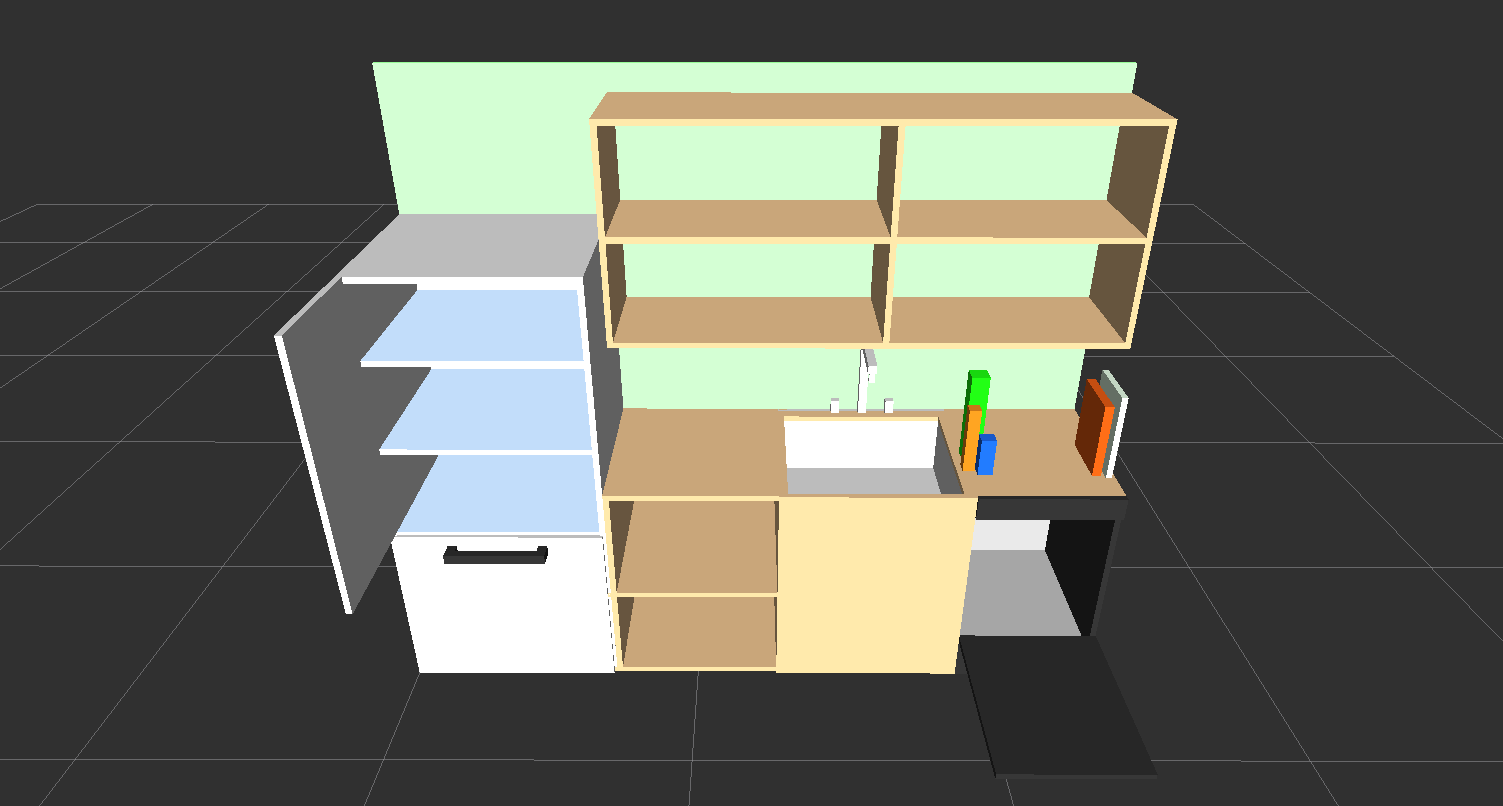
\includegraphics[trim = 70mm 0mm 70mm 0mm, width=0.62\columnwidth, clip=true]{pictures/countertop_scene2}
  \begin{minipage}[b][][s]{0.352\columnwidth}
  \centering
    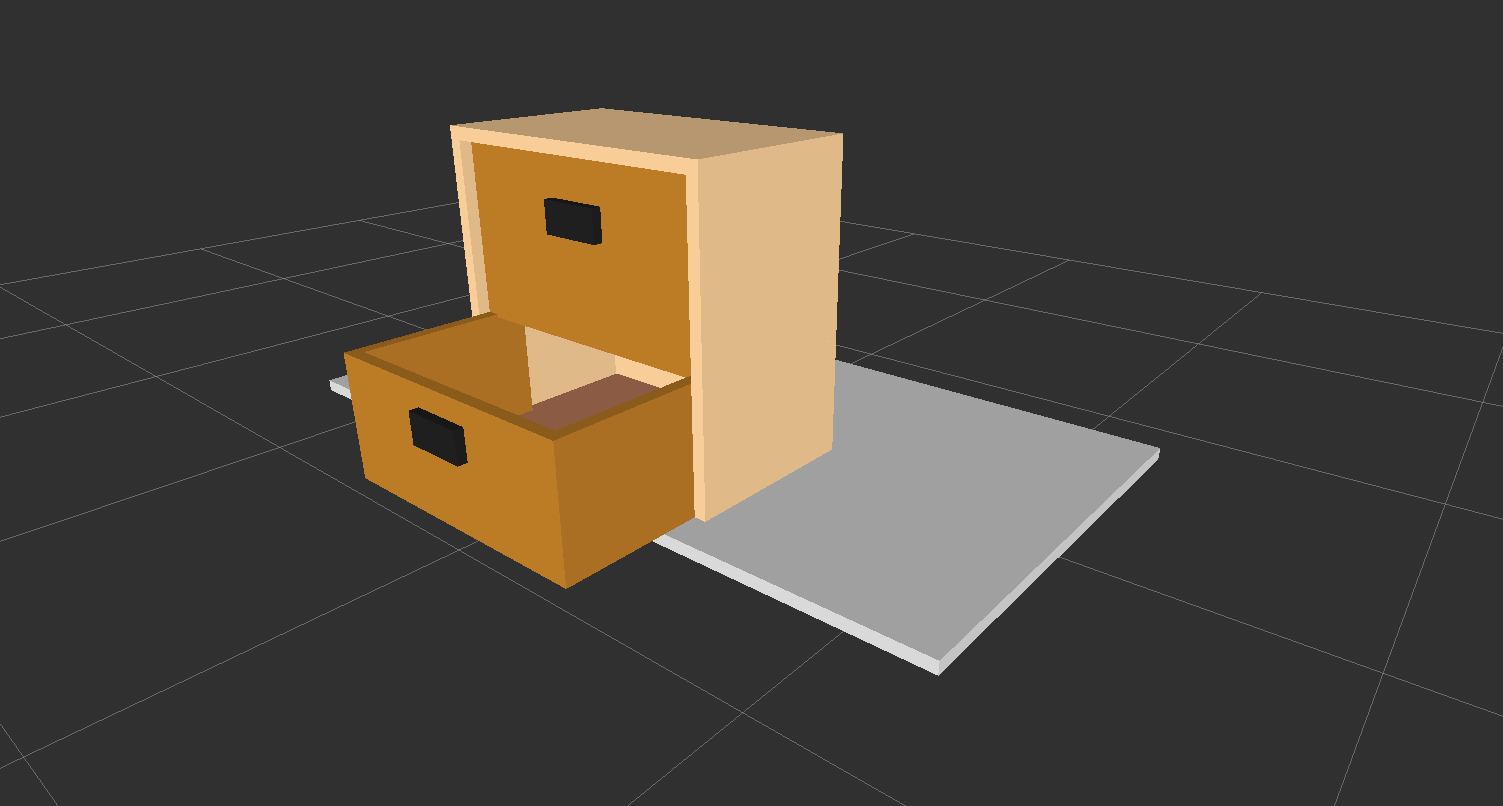
\includegraphics[trim = 70mm 0mm 70mm 0mm, width=\textwidth, clip=true]{pictures/drawer_scene2}
    \vfill
    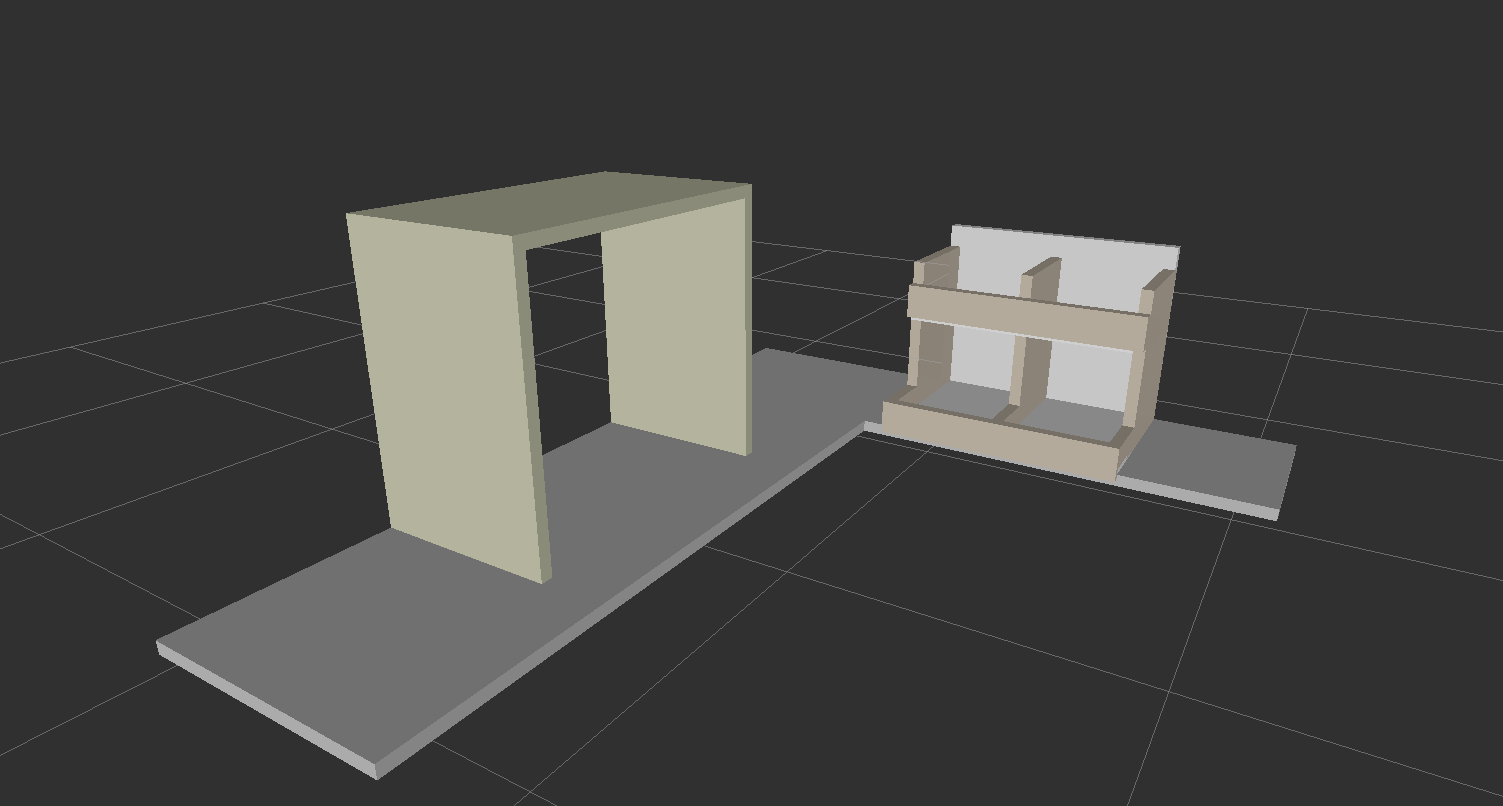
\includegraphics[trim = 30mm 0mm 30mm 0mm, width=\textwidth, clip=true]{pictures/industrial_scene2}
  \end{minipage}
  \hfill
\caption{The scenes used in generating the robot motions to collect feedback from human observers. \emph{Drawer} (top right), \emph{Countertop} (left), and \emph{Industrial} (bottom right)}\label{fig:scenes}
\end{figure}

Robot motion has been primarily influenced by the need to generate smooth jerk-free trajectories for industrial robots that minimize wear and tear of internal parts. In recent years, there has been more interest in the generation of motions for robots working in human environments, i.e. environments with clutter and people working next to the robots. Most attention, though, has been focused on generating {\em collision-free} motions. Examples include the use of randomized planners~\cite{kuffner2000rrt}, trajectory optimization techniques~\cite{Mrinal:2011}, and deterministic search-based techniques~\cite{cohen2010search}. 

Human motions have been the subject of recent study with the intent of determining whether there are certain motor or locomotor invariants that best describe human manipulation or locomotion. Human motion has been observed to be stereotypical~\cite{Atkeson:85}, i.e. learned motion patterns that are repeatedly used. This requires less planning of individual motions and contributes to making human motions more deterministic and predictable. The minimum jerk principle for human motions specifies that the trajectory of the human can best be represented as a motion that minimizes jerk of the hand~\cite{Flash:85}. Uno et. al.~\cite{Uno:89} used minimum torque change as a measure to explain the observed human motions. Minimizing jerk at the joint level~\cite{Rosenbaum:1995} has been another criterion used for human motion. Human motion has also been found to be optimized~\cite{Arechavaleta:2006}. Albrech et. al.~\cite{Albrecht:2011} studied the reaching motions of several subjects in table-setting situations and attempted to codify the motion using cost functions representing minimum-jerk hand motions, minimum-jerk joint motions, minimum torque change and a combination of all three. They found that no single combination of the cost functions explained the observed data completely. 

Recent work has also addressed the task of making motions predictable (similar motions in similar environments and tasks) and/or legible (make it easier for human observers to understand the intent of the robot)~\cite{Beetz:2010}. Legibility makes it possible for human observers to understand clearly what a robot is intending to do, allowing them to modify their actions and motions if necessary. Predictability implies that the robot will always be consistent in its actions, removing the element of surprise for human observers. These concepts have been well-studies recently with the intent of measuring legibility~\cite{Lichtenthaler:2011}, using expressions to improve the readability of robots~\cite{Takayama:2011} and generating anticipation~\cite{Gielniak:2011}. In~\cite{Dragan:2013}, the notion of legibility was incorporated into a constrained trajectory optimization motion planner to generate motions that are more legible to human observers. 

There has been relatively little examination of how human observers perceive robot arm trajectories in environments with obstacles. There is no data available for how human observers react to such robot motions. It is not clear whether minimum-jerk trajectories (or other cost functions) are the best descriptors of motions in such environments or if there are other features that better explain human-observer preferences in such sitations. Our goal in this work is to collect the data needed to answer the query, ``Which robot trajectories in cluttered environments do human-observers prefer'' A second question that we would like to answer is ``Why are certain robot trajectories preferred by human-observers?'' This is a larger question that we aim to address in future work and instead we focus on, ``Can we predict a human-observer preference for a given trajectory'' The answer to this latter question, we hope, will eventually point us towards trajectories that are better accepted by human observers. 

\section{Approach}
\label{sec:survey}
Our approach starts with an online survey designed to get information from multiple users about how well they like robot trajectories. In this section, we will describe in detail the infrastructure used to create the trajectories and movies that were used in the survey. We will also describe the online survey procedure in detail. 

\subsection{Planning System Infrastructure}

\begin{wrapfigure}[13]{l}{.5\linewidth}
\centering
  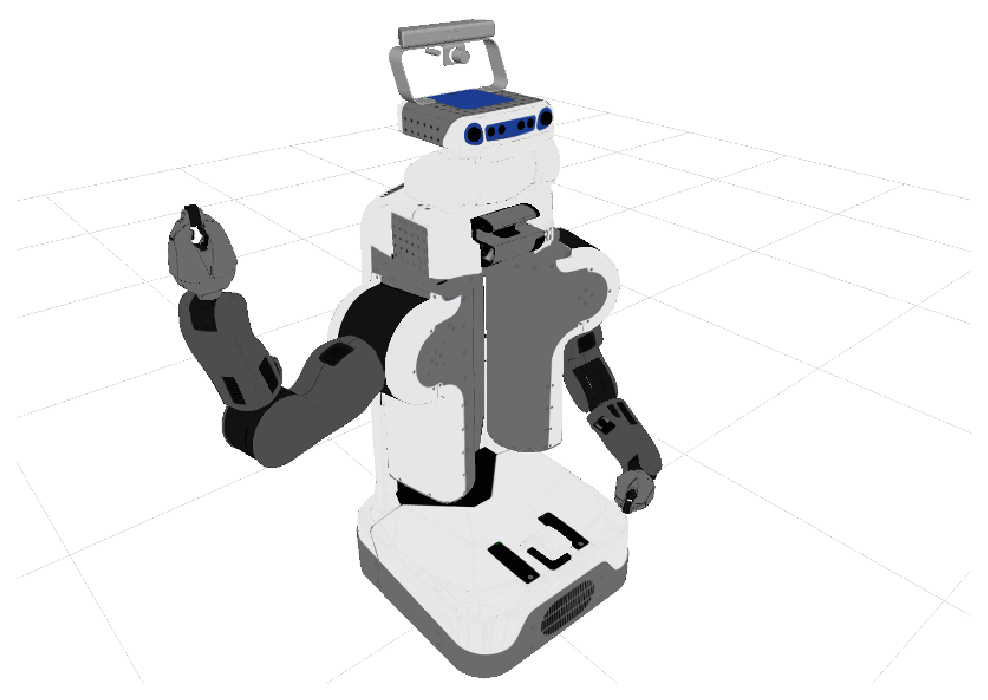
\includegraphics[trim = 0mm 0mm 40mm 0mm, width=0.5\columnwidth, clip=true]{pictures/pr2_robot_4_downscale}
\caption{{\footnotesize PR2 robot.}}
\label{fig:PR2}
\vspace{0.1in}
\end{wrapfigure}

We extended the MoveIt! benchmarking architecture~\cite{cohen2012generic} with video generation capabilities to automate the generation of a large number of trajectories. The MoveIt! architecture allows for the definition of environments, referred to as planning scenes, start and goal states for robots (motion planning queries). It also allows for the use of any supported planning algorithms (planners). A combination of different scenes, motion queries, and planners was used to generate robot trajectories for evalutation. We chose three distinct scenes (Fig.~\ref{fig:scenes}): a kitchen (Countertop), an industrial workbench (Industrial) and a drawer on a table (Drawer). Multiple queries were generated in each scene for trajectories of the right arm of the PR2 robot (Fig.~\ref{fig:PR2}. The robot was positioned in the scenes manually and motion planning queries were constructed by hand. The positioning in the scenes was done with the expectation that the planning queries would not be impossible or trivial for the planning algorithms to solve. 

\begin{table*}[t]
\centering
\scalebox{0.9}{
\begin{tabular}{|c||c|c|c|c|c|c|c|}
\hline
Efficiency  & Highly inefficient& Moderately inefficient& Slightly inefficient& Neutral & Slightly efficient& Moderately efficient& Highly efficient\\
\hline
Elegance    & Highly awkward& Moderately awkward& Slightly awkward& Neutral & Slightly elegant& Moderately elegant& Highly elegant\\
\hline
Smoothness  & Highly rough& Moderately rough& Slightly rough& Neutral & Slightly smooth& Moderately smooth& Highly smooth\\
\hline
Overall     & Extremely poor& Moderately poor& Somewhat poor& Neutral & Somewhat good& Moderately good& Extremely good\\
\hline
\end{tabular}
}
\caption{The four rating categories/attributes and the associated scales for each presented to the survey respondent.}
\label{tab:rating_scales}
\end{table*}

%\begin{figure}[b]
%    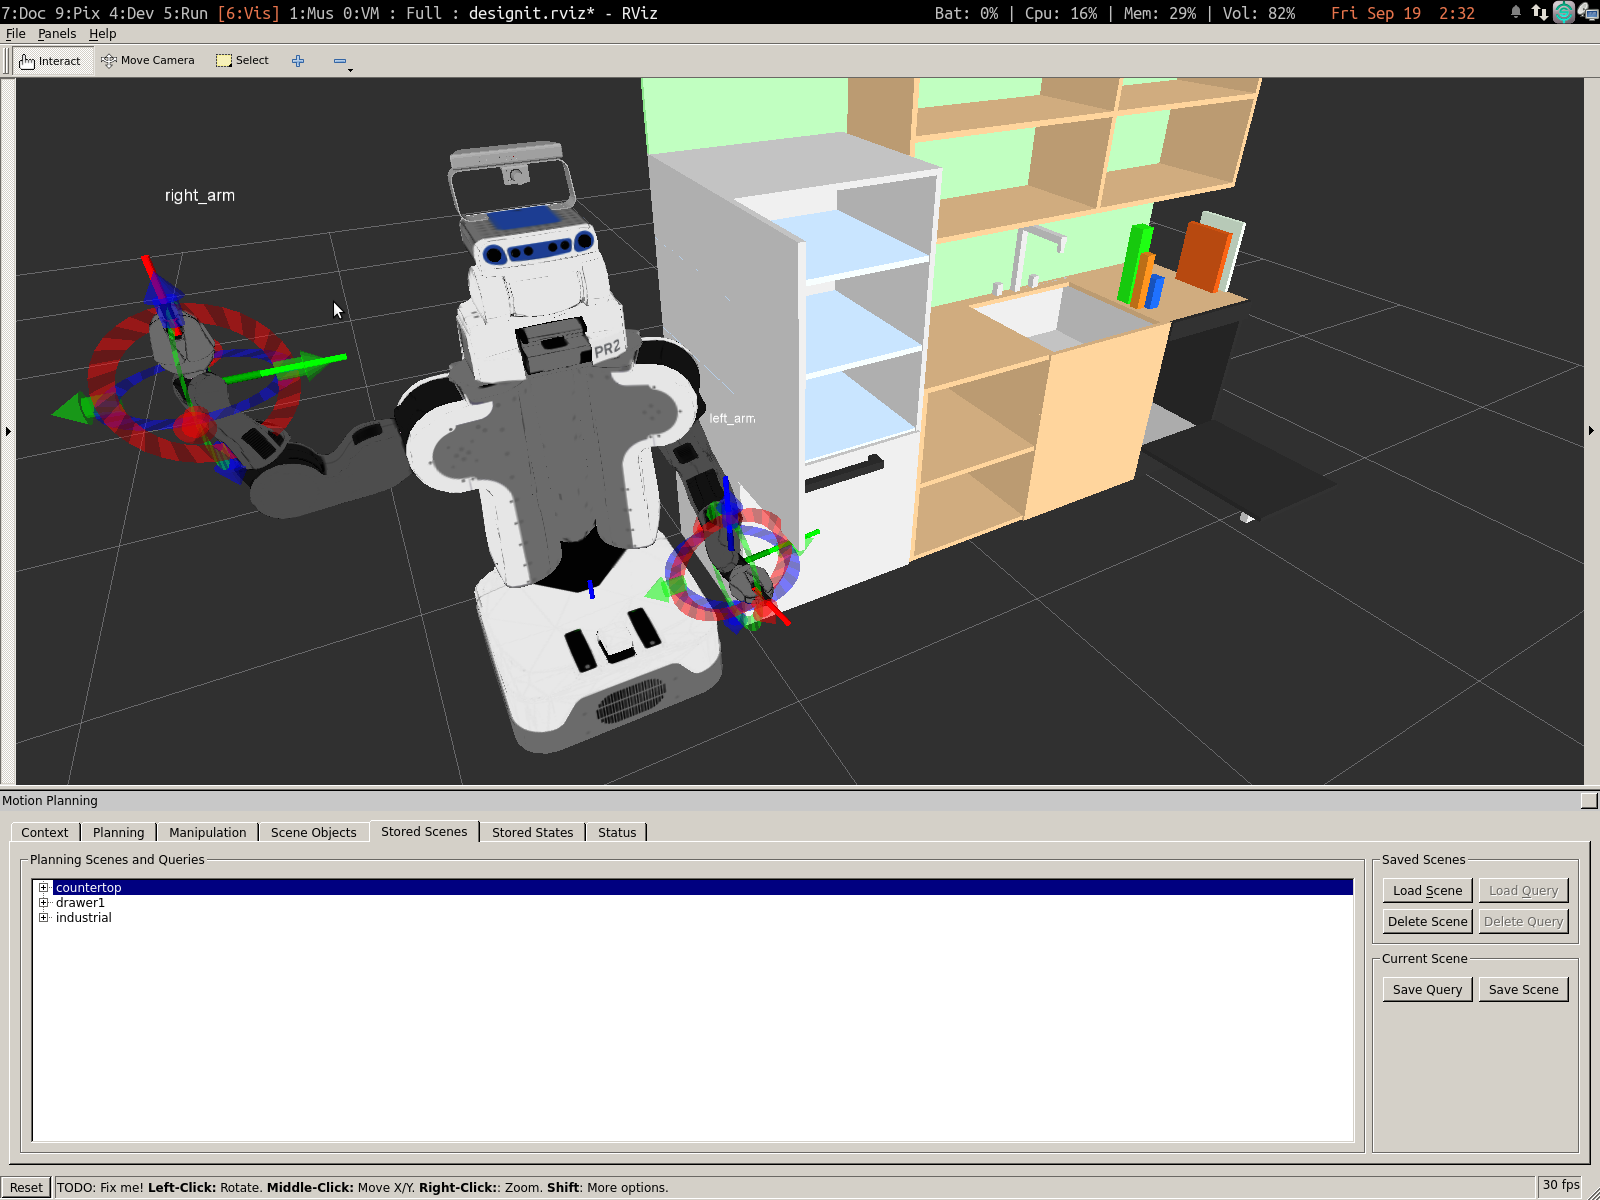
\includegraphics[trim = 0mm 0mm 0mm 0mm, width=\columnwidth]{pictures/designing_queries_moveit}
%    \caption{Screenshot of the planning query design process which involved hand-picking start and goal query poses for the various scenes manually to ensure they were neither trivial nor impossible for the planning algorithms to solve. This was accomplished through use of RVIZ and interactive markers.}
%    \label{fig:design}
%\end{figure}

The planning algorithms that we used are RRT-Connect~\cite{kuffner2000rrt} and RRT*.  RRT*~\cite{frazzoli-RRTstar} was used with two different cost functions: PathLength and MaxMinClearance.The objective for PathLength minimizes the length of the trajectory (as the sum of the euclidean distances between ends of trajectory segments). The objective for MaxMinClearance computes uses the minimum clearance of a configuration belonging to a trajectory as the value it is trying to maximize. Both planners are implemented in the OMPL library~\cite{OMPL:2012}. All the paths generated by RRT-Connect are shortcutted for a finite amount of time to improve the quality of the paths. The planned trajectories are post-processed by an iterative-time parameterization method that time-parameterizes the trajectories while taking into account velocity and accelerations. The infrastructure we designed around MoveIt! allows us to automatically generate movies of the generated trajectories using the ROS Visualizer (Rviz). We generated movies from different viewpoints to maximize the visibility of the motion to human observers reviewing it. A total of 103 different trajectories were generated in this manner. 

Our main focus in generating trajectories was to generate a wide sample. The choice of planners used to generate the trajectory was not important. We preferred the randomized planners since they natively generate a wide variety of plans that are less likely to be similar to each other. We could have chosen to generate all our trajectories with an  asymptotically optimal planner like RRT* but we would not have been able to generate a variety of plans. This would also have restricted the richness of the trajectory features we could work with. Our intent in this work is not to evaluate particular planning algorithms but instead to examine the preference that human-observers have for generated trajectories regardless of the methods used to generate them. 

\subsection{Online Survey}

We conducted an online survey\footnote{The online survey was conducted after gaining a waiver from SRI's IRB after a review of our survey procedure. Our survey followed standard guidelines for privacy of respondent information when conducting a survey on Mechanical Turk.} where we asked human observers to rate a variety of trajectories of the PR2 robot. The survey was built on Amazon's Mechanical Turk, which has become a useful tool for large online data gathering and crowd-sourced work. Each respondent in the survey was presented with a set of demographic questions, a video, and asked to rate the robot's motion on the attributes  of elegance, efficency, smoothness and overall impression (a summary of the rating scales used in the main survey question can be seen in Table~\ref{tab:rating_scales}). The ratings were later converted into numerical values on a scale of 1 to 7. Each respondent was expected to rate multiple trajectories but could not rate a trajectory more than once. Each video has four different views of the robot displayed simultaneously. Respondents were asked demographic questions about familiarity with video games, familiarity with robotics, age group and highest education level. The demographic information was not used to filter the responses we collected.  

Mechanical Turk allows monetary compensation on completion of the survey, which we set to 15\textcent~per survey. We estimated the time that each respondent would take to rate a single trajectory as 1-2 minutes. Additionally, the respondents were allowed to replay the trajectory video repeatedly. The maximum possible payout for each respondent is thus 15.45\$ (if each survey took 1.5 minutes to complete then the wage is approximately 6\$ per hour). This is standard compensation for quality work on Mechanical Turk for tasks of this type, as was pointed out to us by several veteran Mechanical Turk surveyors. 

Respondents on Mechanical Turk are only paid if the survey organizer approves their response. A control question, asking the respondent to identify the known action of a robot in a video, served as the first satisficing trap to ensure that respondents were truthfully attempting the survey (see~\cite{krosnick1996satisficing} for more information on satisficing in survey responses). Survey responses were also manually examined to assess whether respondents were responding honestly. We looked at whether respondent responses were outliers when compared to the rest of the group. We also examined the average time taken by each respondent to complete the survey. Overall, we found that all the respondents had made a honest attempt at filling out the rating and we did not reject any responses. 

%\begin{figure}
%    \frame{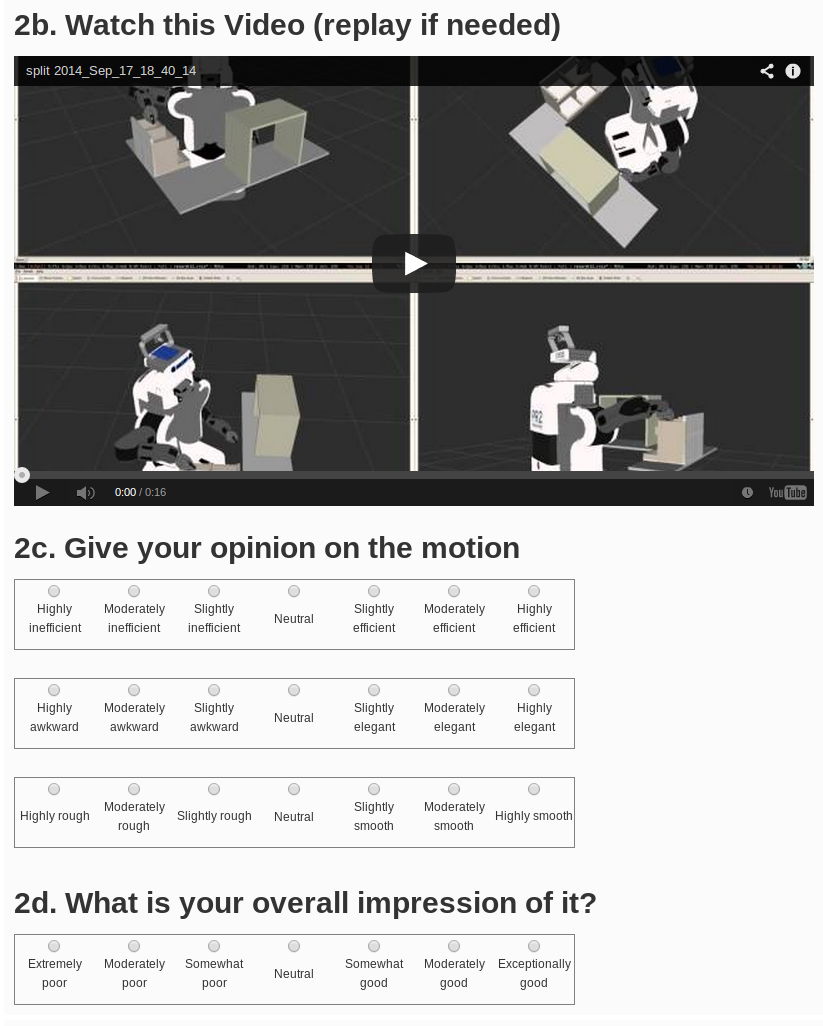
\includegraphics[trim = 0mm 0mm 0mm 0mm, width=\columnwidth]{pictures/amazon_survey_screenshot}}
%    \caption{The main survey question which prompts the respondent for a rating in four motion characteristics (efficiency, elegance, smoothness and overall impression) after presenting a video that demonstrates the motion from four clearly visible vantage points for any sample trajectory.}
%    \label{fig:survey_question}
%\end{figure}

%\begin{figure}
%\frame{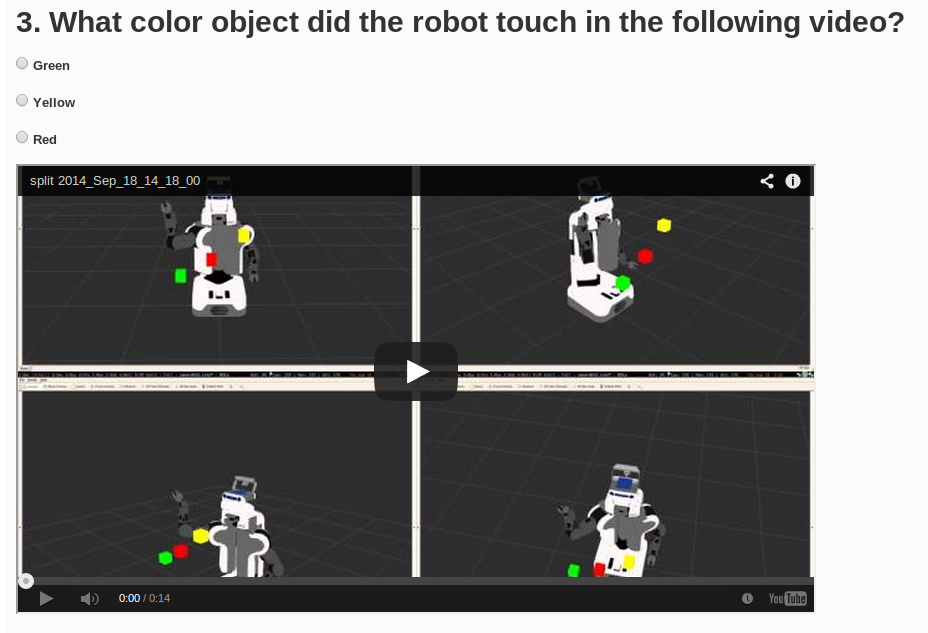
\includegraphics[trim = 0mm 0mm 0mm 0mm, width=\columnwidth]{pictures/amazon_control_question}}
%\caption{The survey control question which prompts the respondent about the action of the robot in the accompanying video. The question we adopted was to ask the particpant which colored cube the robot touched.}
%\label{fig:control_question}
%\end{figure}

\section{Survey Results and Analysis}
\label{sec:raw_results}
The survey resulted in at least 20 ratings for each trajectory (so there were a total of 2060 ratings from participants in the survey). In this section, we will first analyze the raw results from the survey (which are interesting in themselves). Subsequently, we will present a set of features that were used to represent individual trajectories. These features will be used in the next section to learn the human-observer ratings for robot trajectories. 
\subsection{Raw Survey Results}
\begin{figure}[h]
  \centering{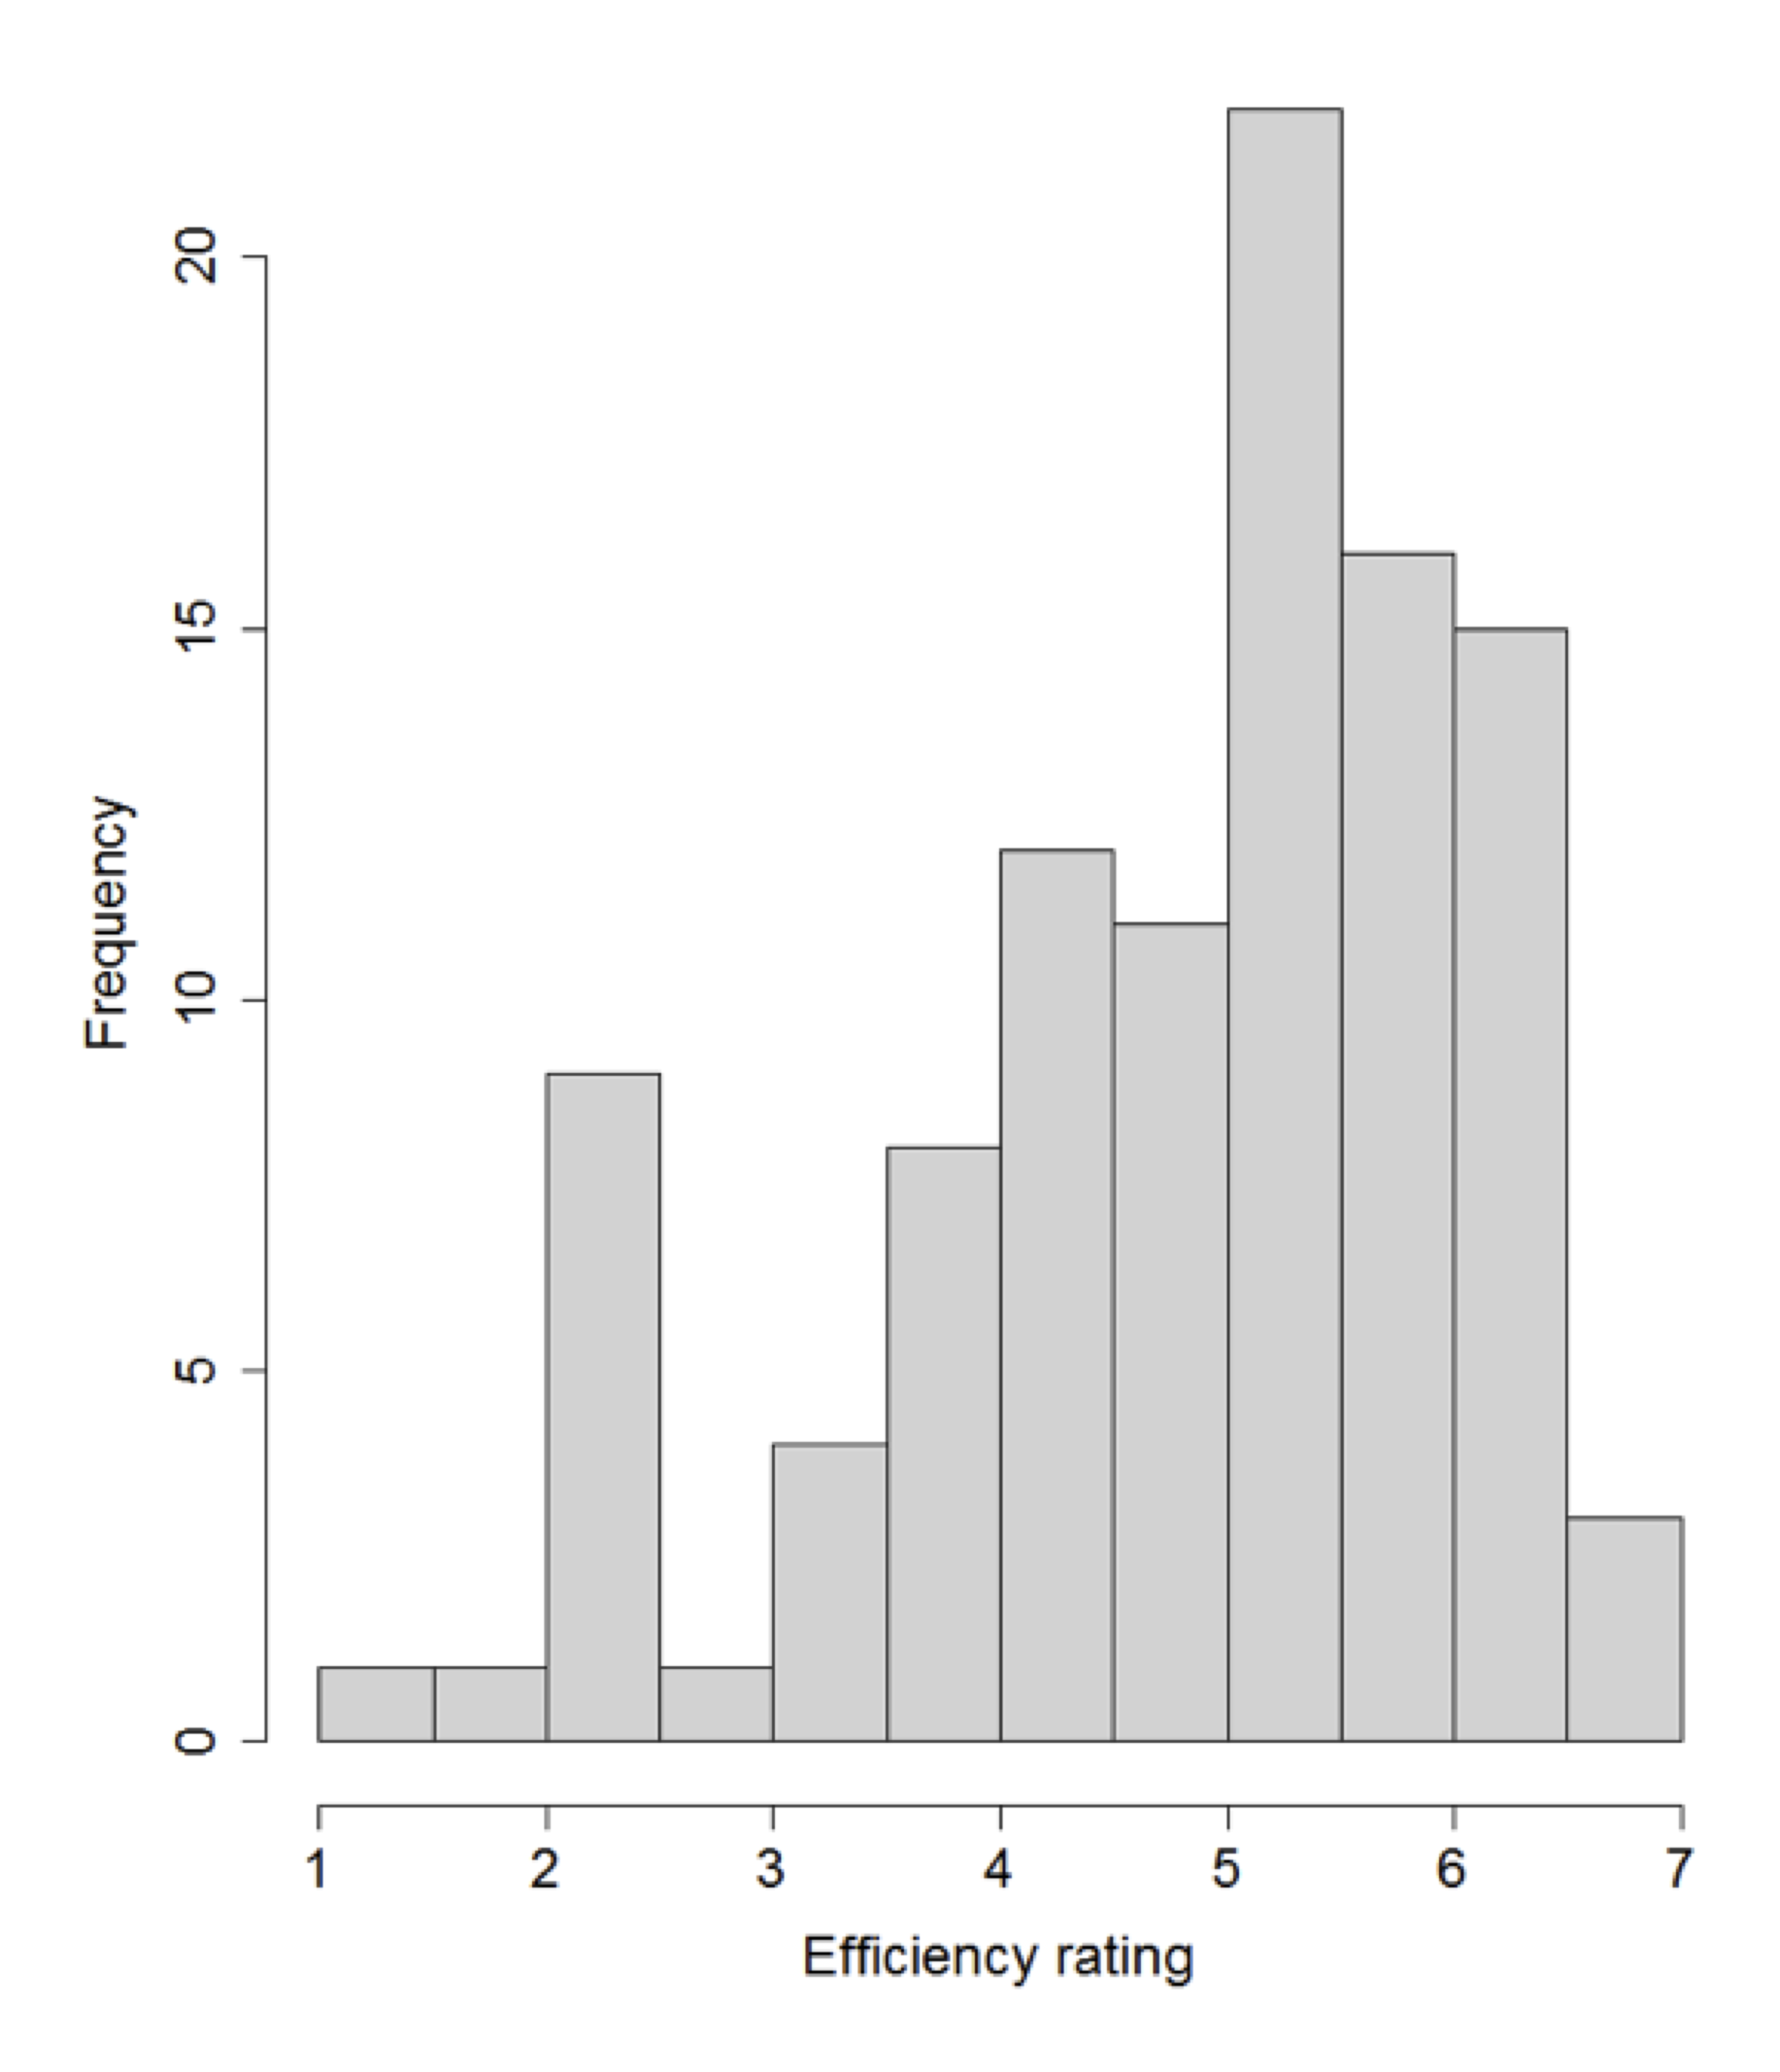
\includegraphics[width=0.45\linewidth]{pictures/efficiency}}
  \centering{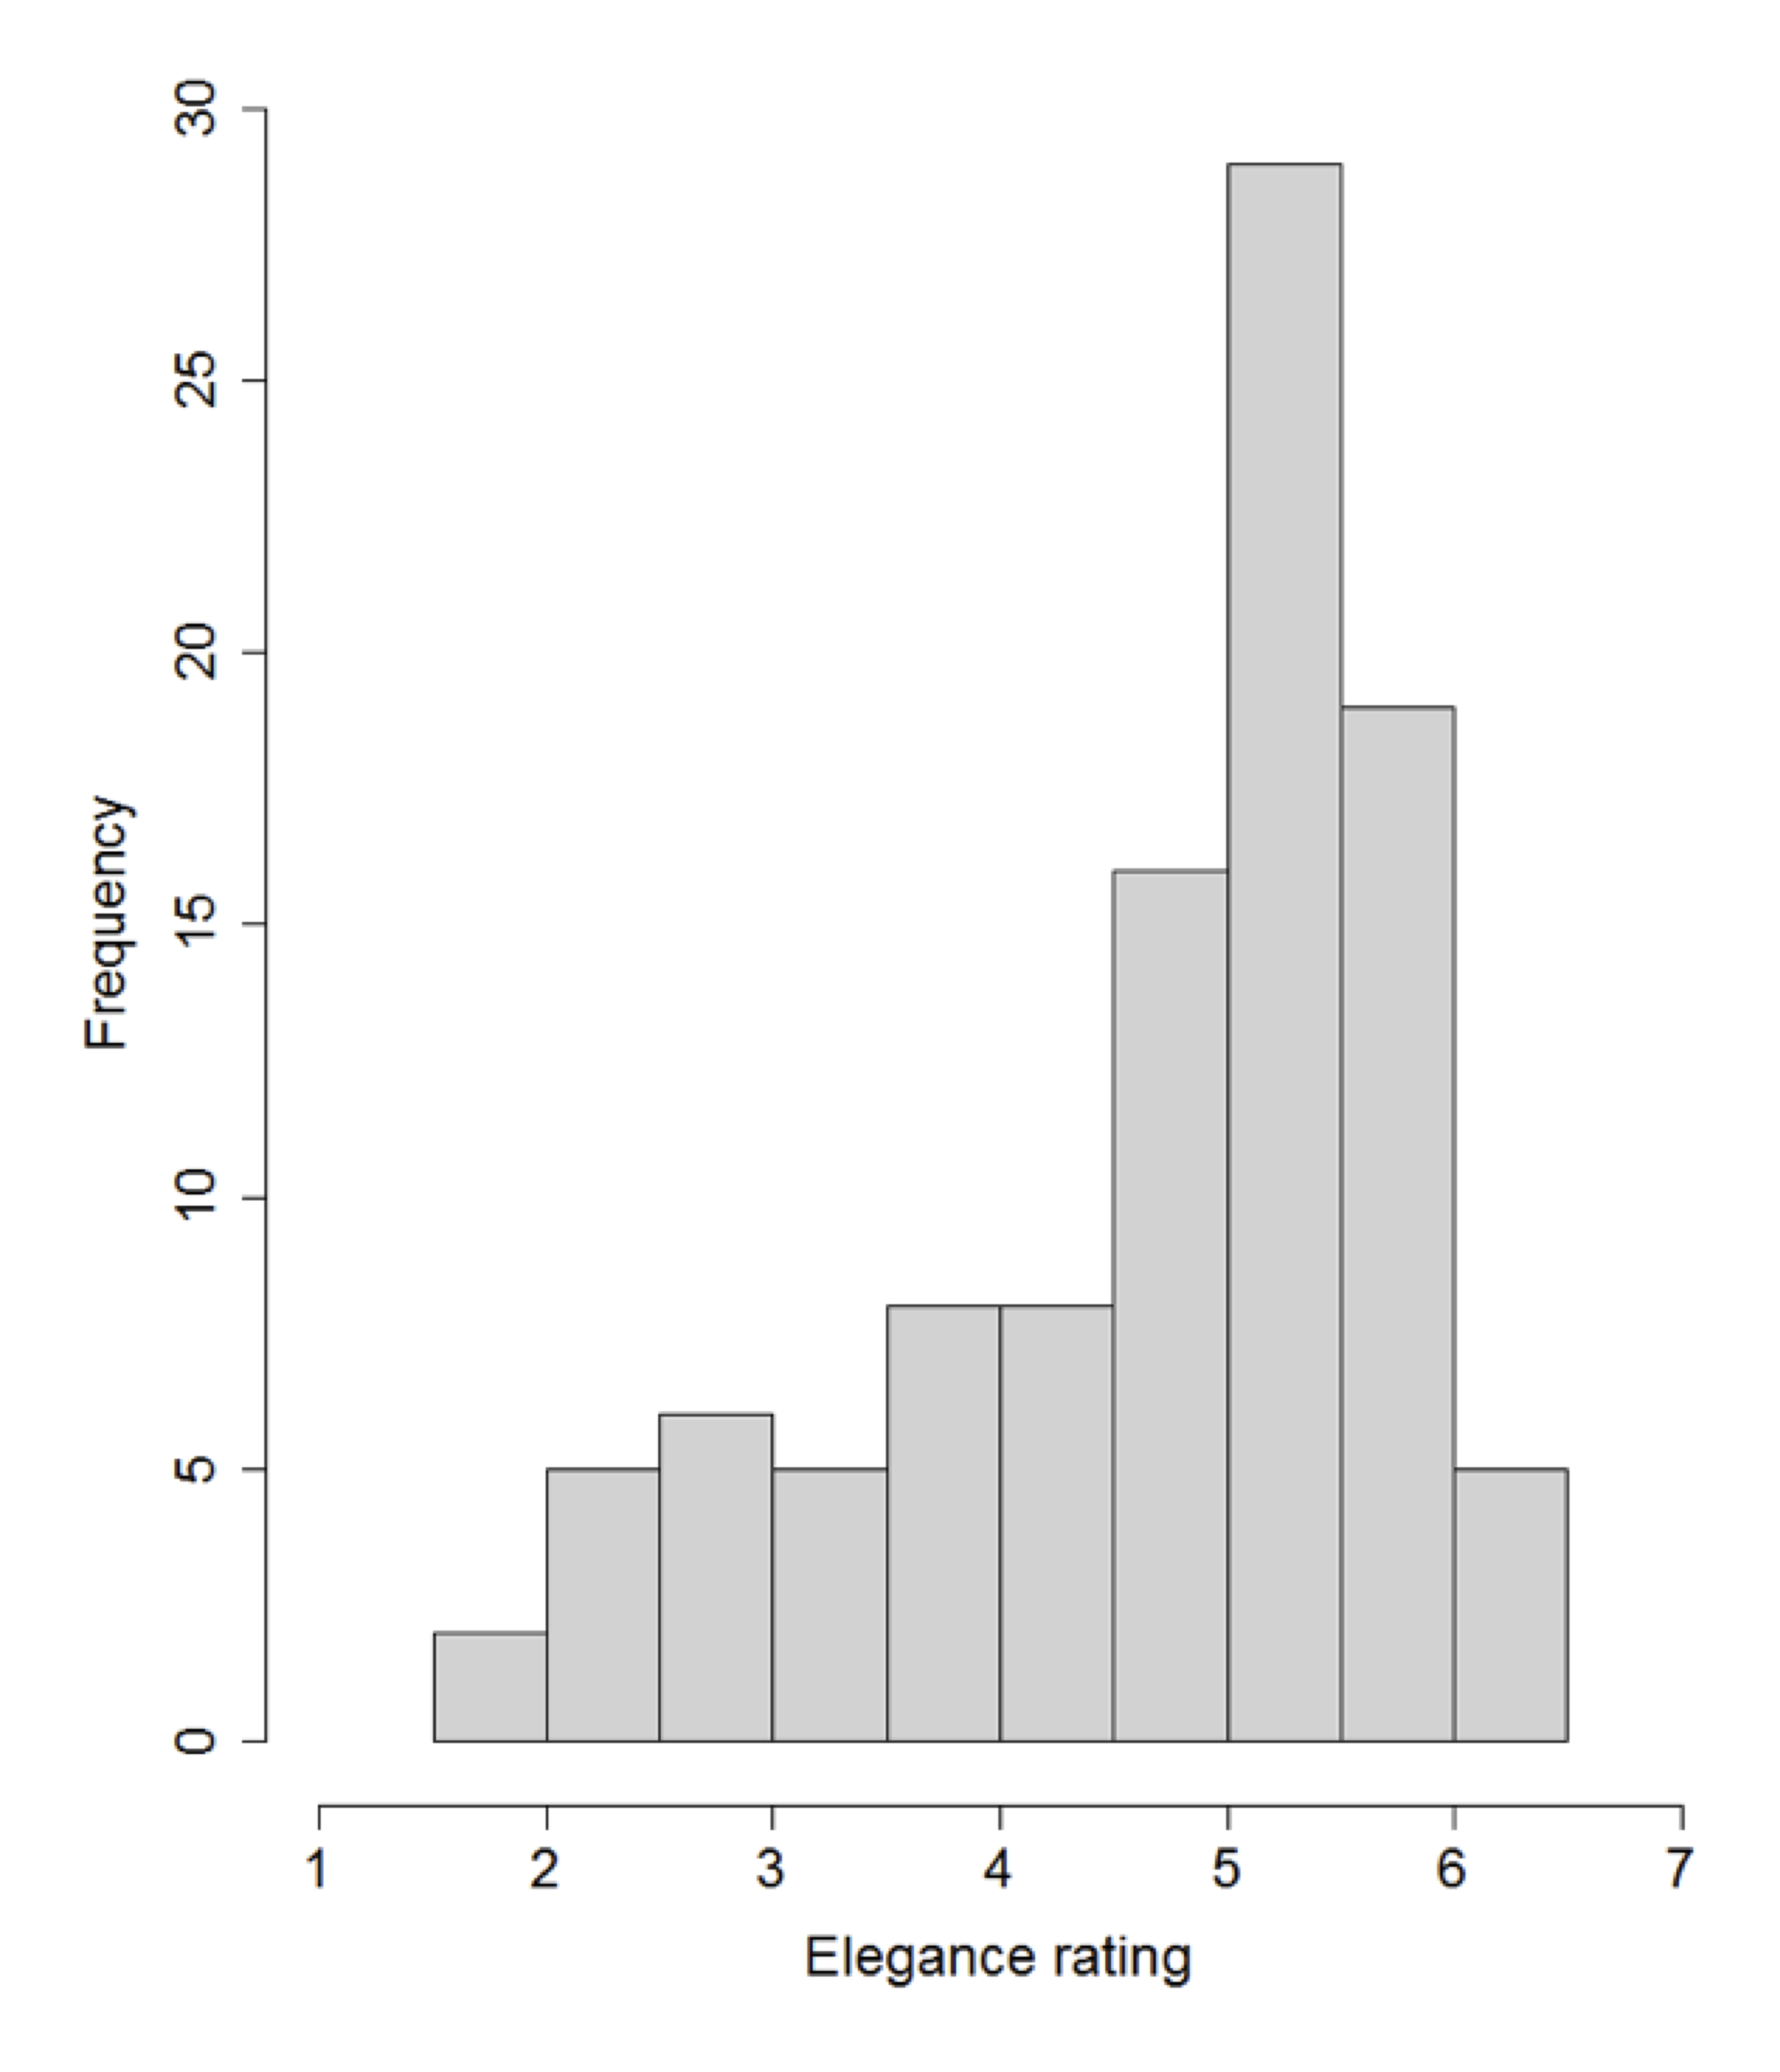
\includegraphics[width=0.45\linewidth]{pictures/elegant}}
  \centering{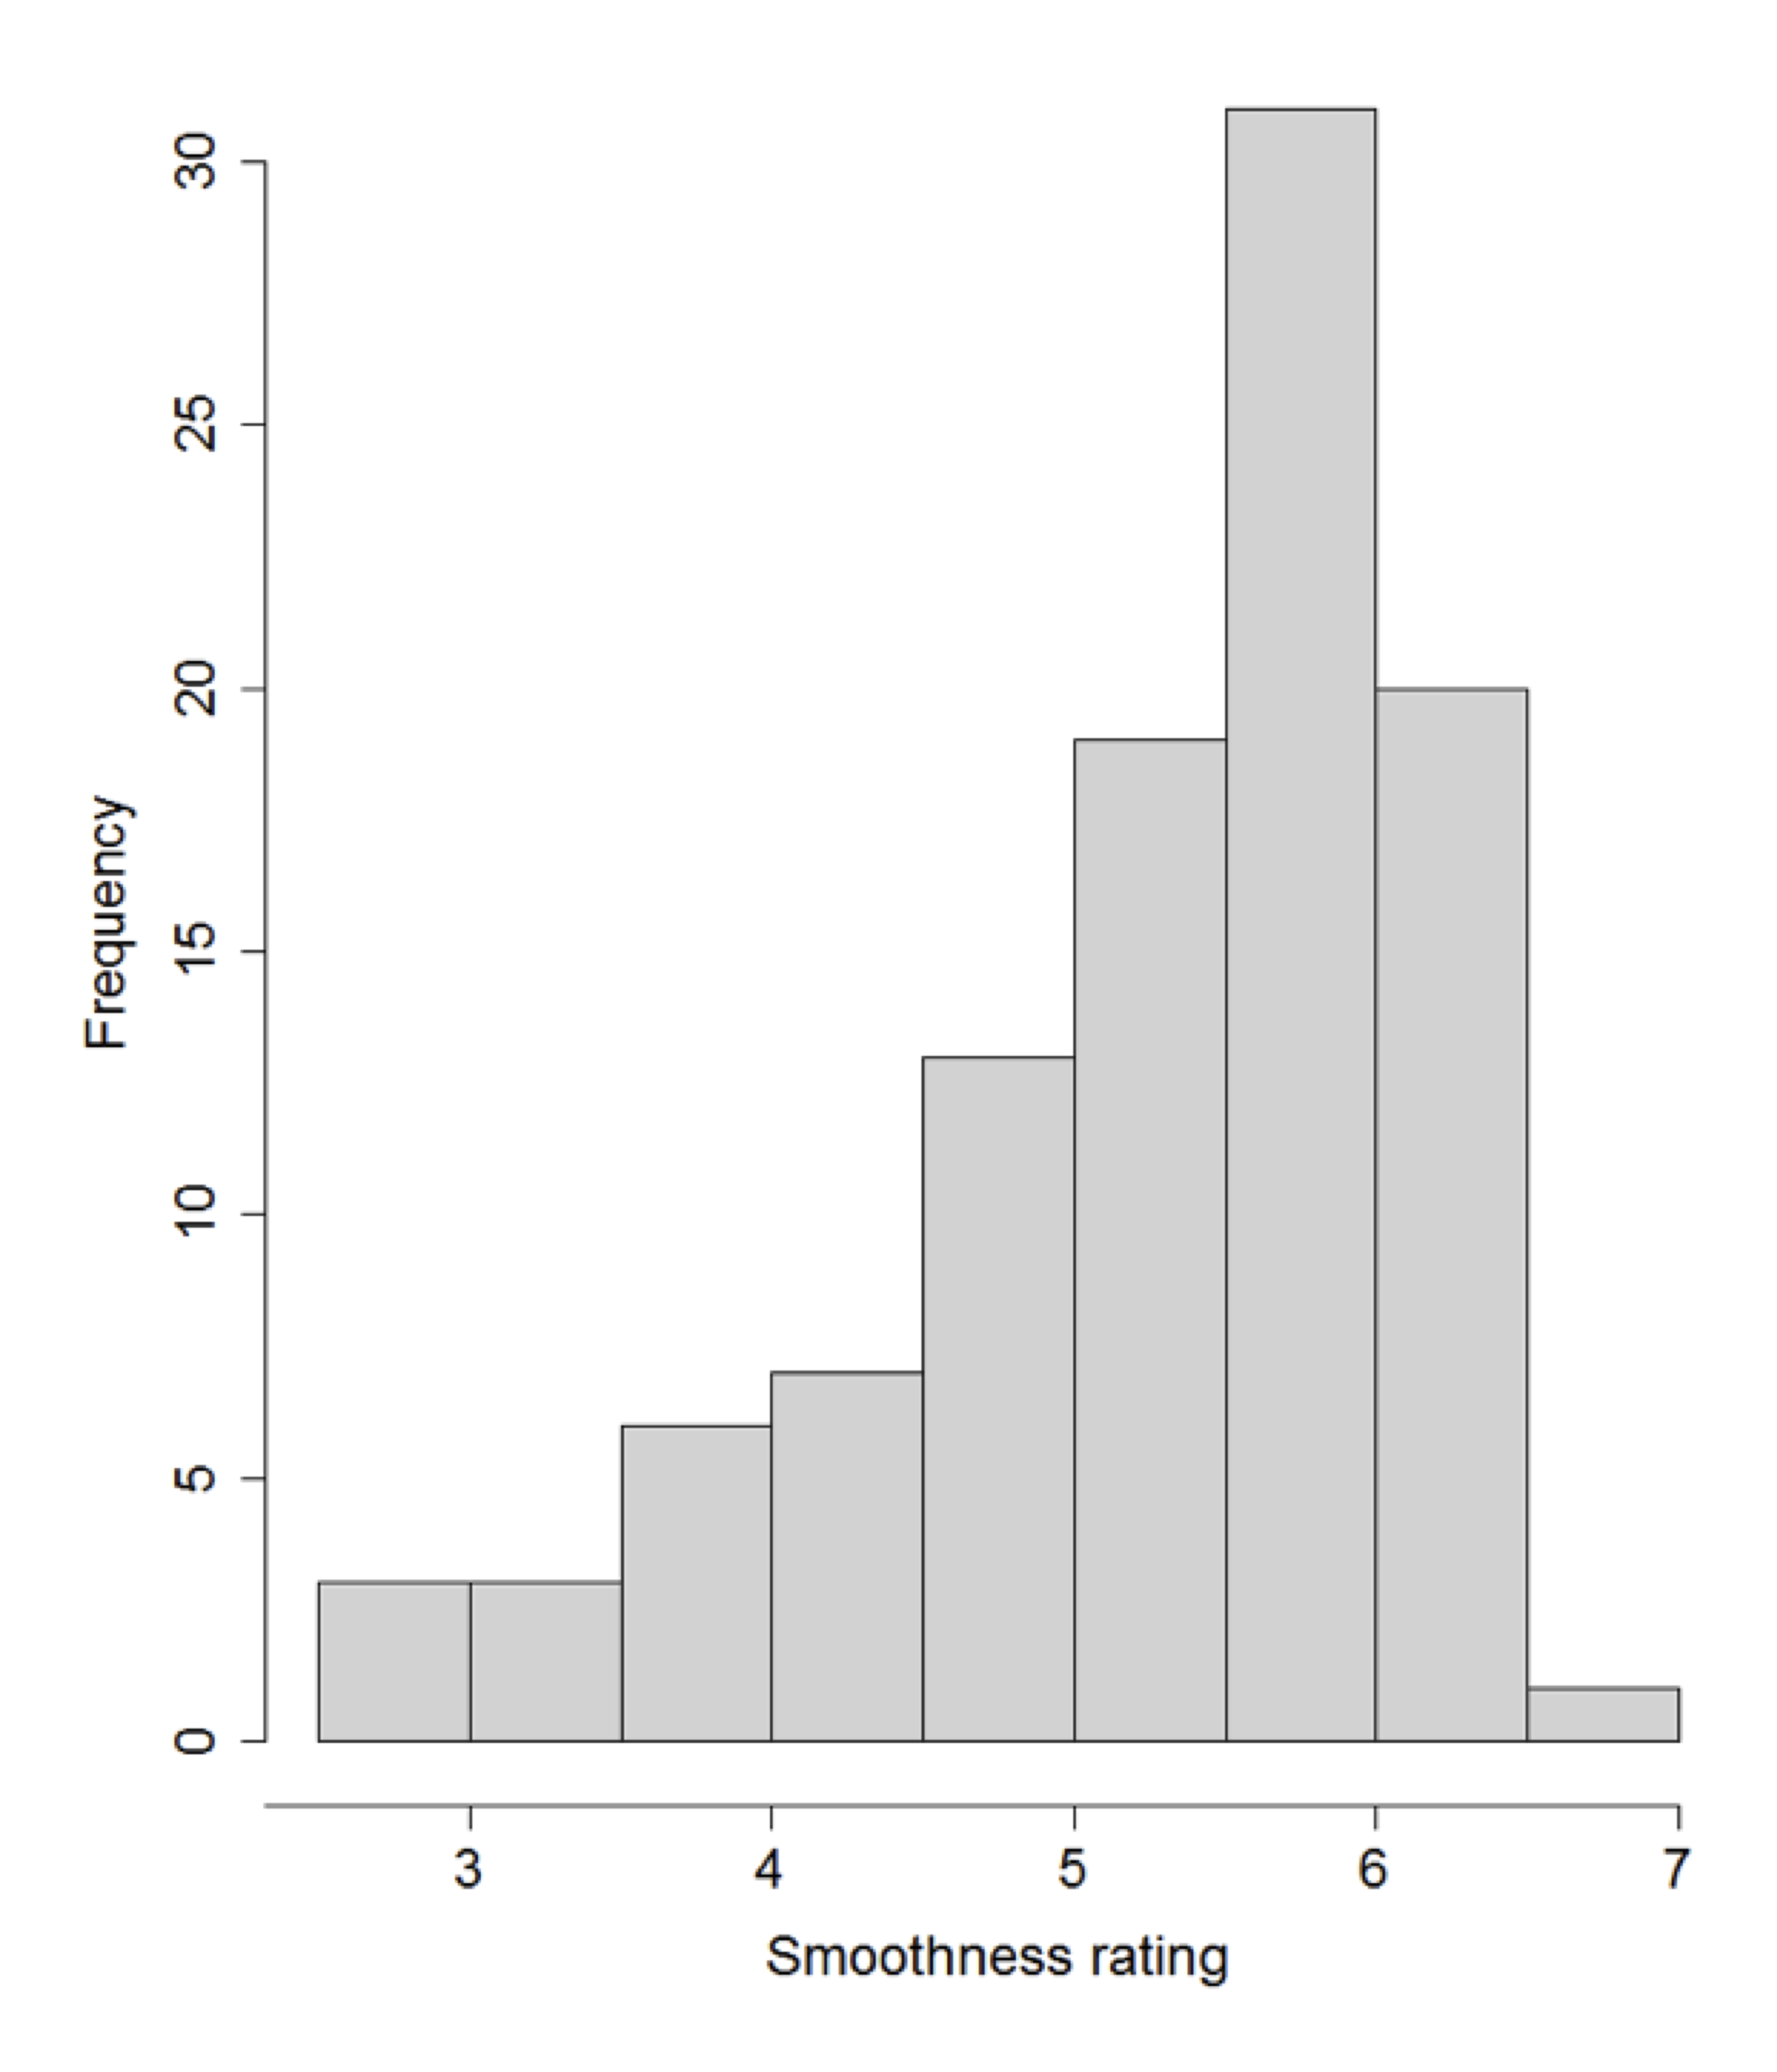
\includegraphics[width=0.45\linewidth]{pictures/smooth}}
  \centering{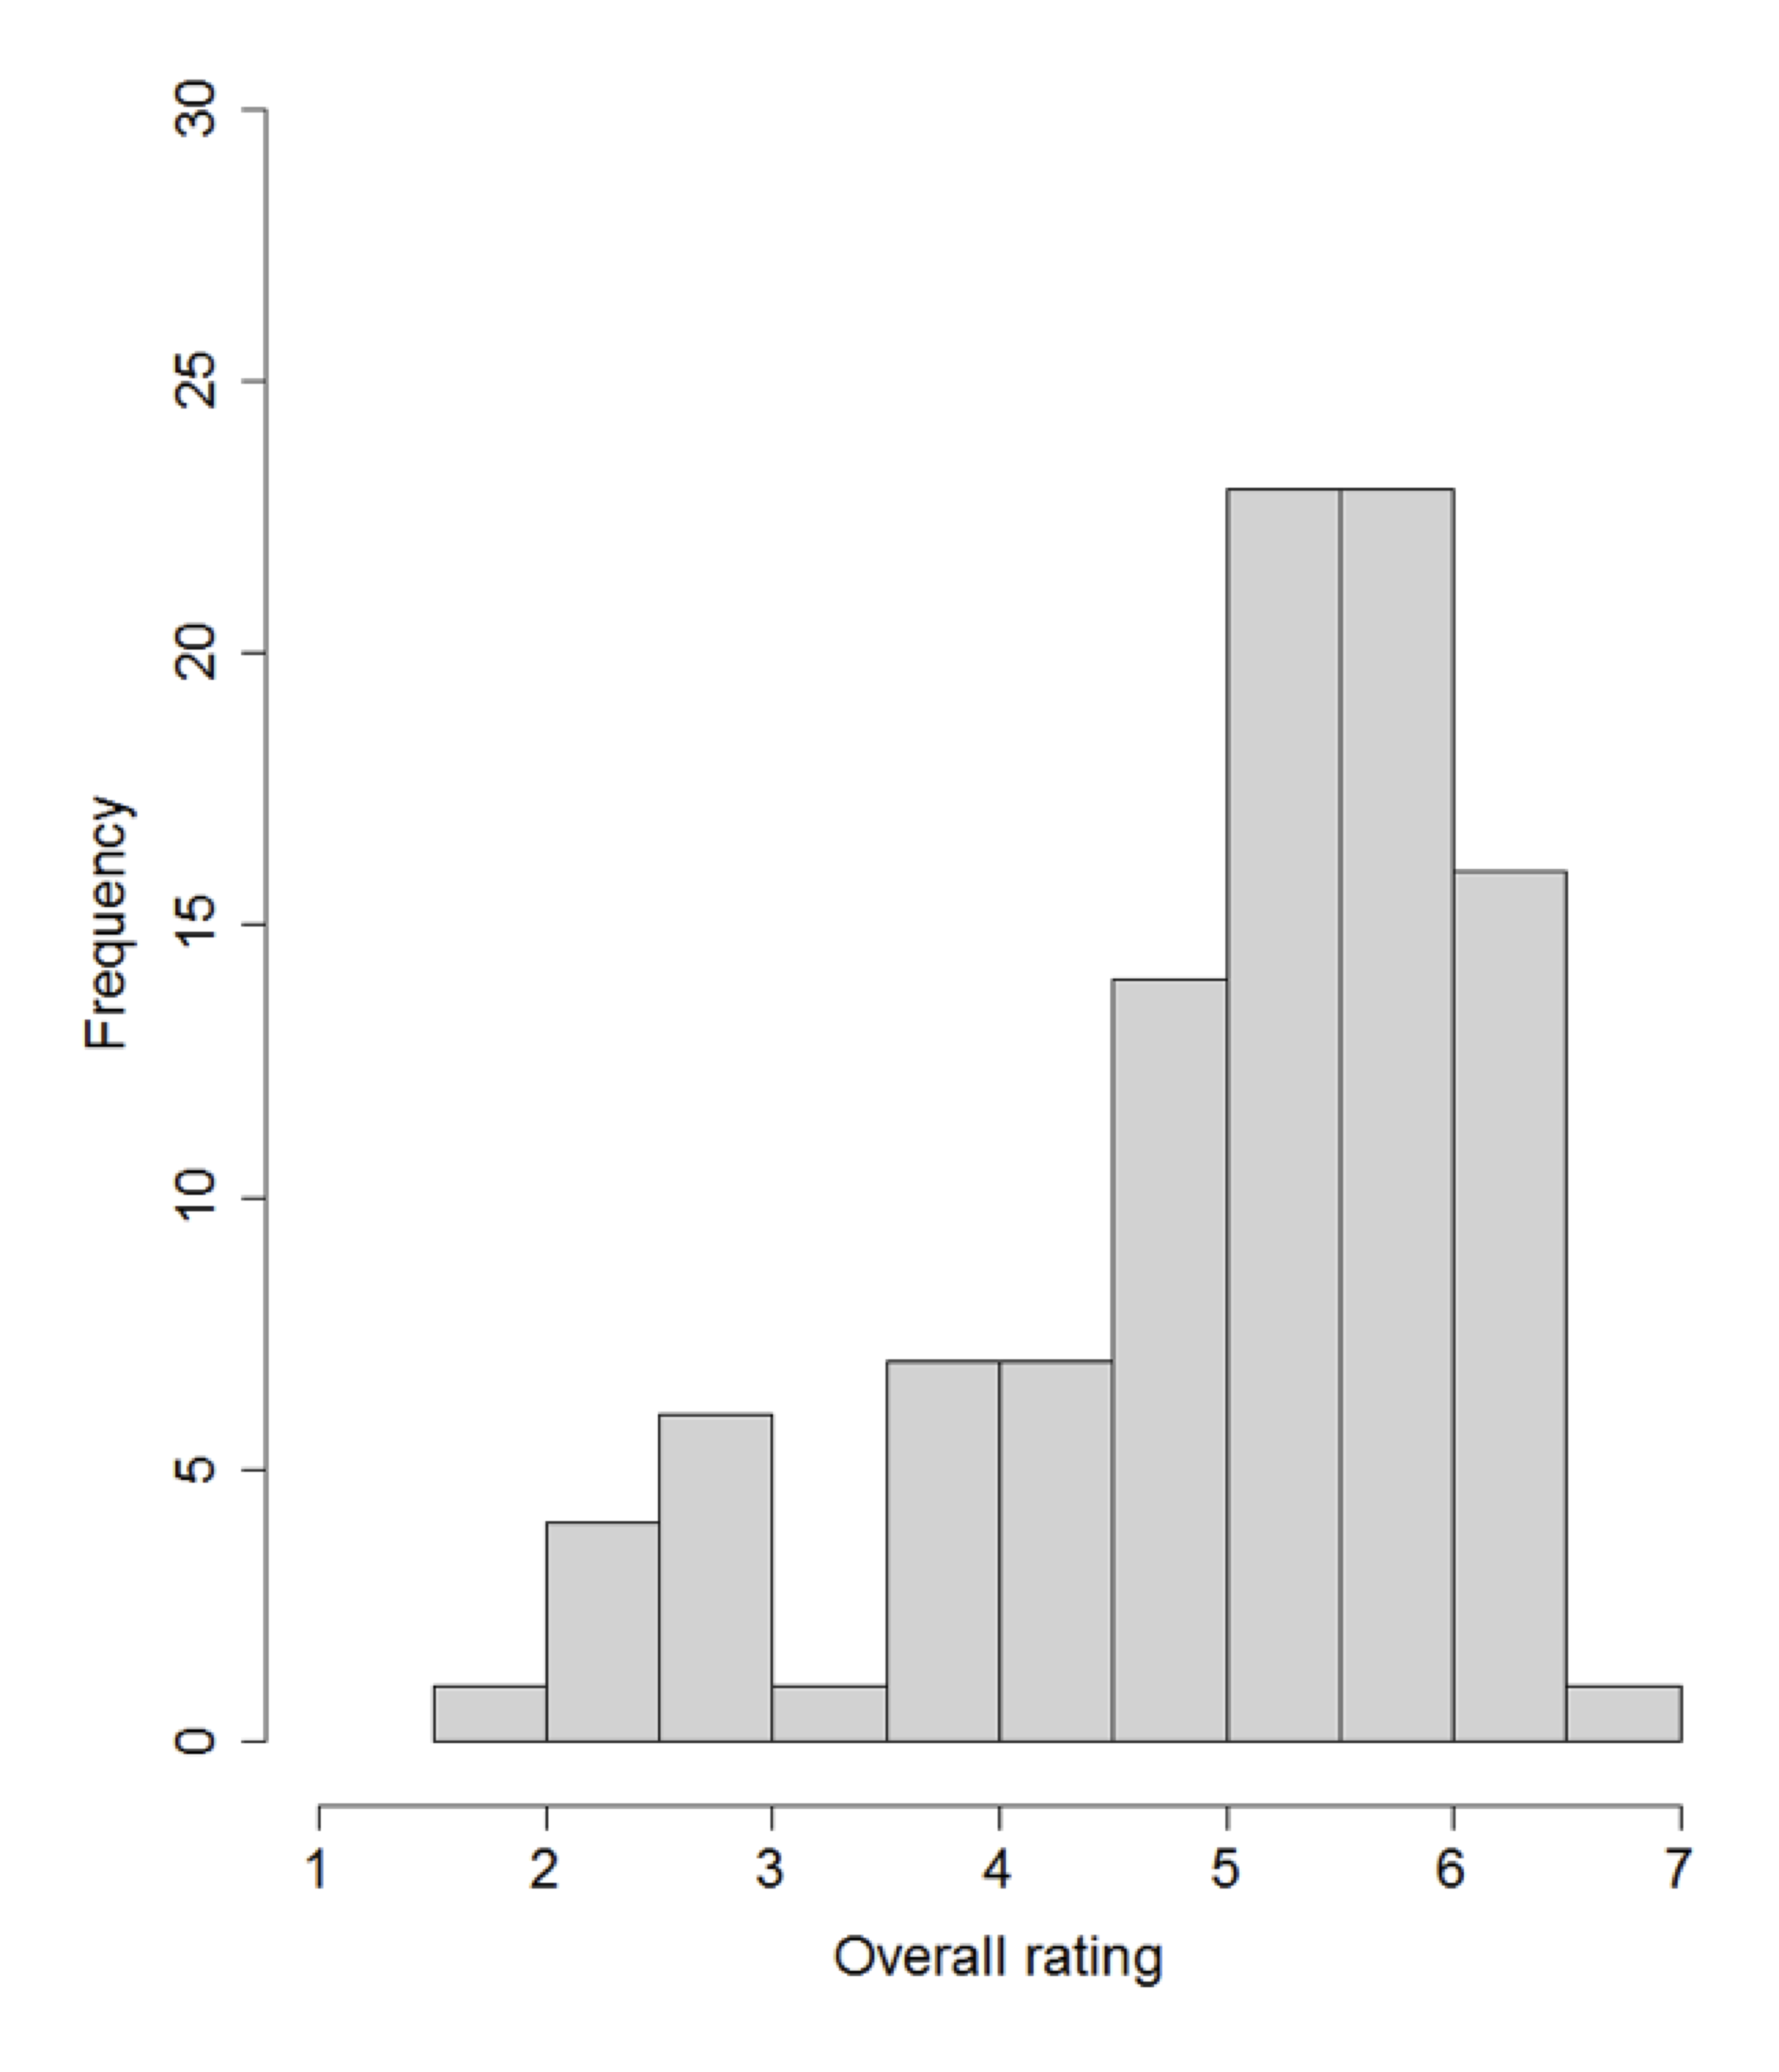
\includegraphics[width=0.45\linewidth]{pictures/overall}}
  \caption{Histogram of averaged ratings for the 103 different trajectories. Clockwise from top left: Efficient vs. Inefficient, Elegant vs. Inelegant, Smooth vs. Rough, Overall Rating}
\label{fig:survey_raw}
\end{figure}
The raw results of the survey are summarized in Fig.~\ref{fig:survey_raw} which shows a histogram of averaged responses for each of the four survey questions across the 103 trajectories that were rated by users. It is clear that a majority of the trajectories in our survey were well received by the human observers but there were quite a few trajectories that were rated badly as well. An analysis of the ratings for each trajectory showed that four (averaged) ratings for each individual trajectory were always similar to each other, indicating that users had similar preferences for each trajectory regardless of the individual attributes used to describe the preference for the trajectory (efficient, elegant, smooth, overall). Table~\ref{tab:correlation} shows the Pearson's correlation coefficients corresponding to pairs of attributes. Attributes across individual questions are highly correlated at a statistically significant level of 1\% (with p-values $< 0.01\%$). The 95\% confidence intervals for all the four ratings for each trajectory was less than 1.0. 
\begin{table}
\centering
\begin{tabular}{|c|c|c|c|c|}
\hline
& Efficient & Elegant & Smooth & Overall \\ \hline
Efficient & 1 & 0.96 & 0.91 & 0.98 \\ \hline
Elegant & 0.96 & 1 & 0.96 & 0.98 \\ \hline
Smooth & 0.91 & 0.96 & 1 & 0.96 \\ \hline
Overall & 0.98 & 0.98 & 0.96 & 1 \\ \hline
\end{tabular}
\caption{Correlation between the four attributes in the survey.}
\label{tab:correlation}
\end{table}

\subsection{Trajectory Features}
\label{subsec:traj_feat}

We identified and computed multiple types of trajectory features. The first set of features we compute for each trajectory take into account the environment around the robot, the shape of the trajectory and the dynamics of the trajectory. These make up our unary features computed only on the input trajectory. We also include features that compare each trajectory to a nominal trajectory - these feature serve to characterize how much the trajectory deviates from the ``expected'' path. We go over these comparative features in the next section. First, we detail the features we computed on each trajectory \tj{} with waypoints $q_i$ where $i={0,\mathellipsis,n}$ and $n=|\tj{}|$. Note that our features are generic, i.e. they can be computed in the same manner for any robot arm trajectory. We believe that our methods should be easily extensible to robots other than the PR2 as well and individual trajectory classifiers could be built for each different robot arm in a similar manner.  

{\bf Path length:}
%The length of the trajectory \tj{} computed as the sum over trajectory segments of the euclidean distance between end points of the segment, or
%\begin{equation}
%\text{Length} = \sum_{i=0}^{n-1} \| q_\text{i}-q_\text{i+1} \|
%\end{equation}
We compute path length for the joint-space trajectory and for three workspace trajectories for the elbow ($\xi_\text{elbow}$), wrist ($\xi_\text{wrist}$) and finger-tip ($\xi_\text{tip}$) links of the right arm (the moving arm). We also compute the length of the trajectory in angular distance by summing over the waypoints $\arccos( \langle Q_\text{i},Q_\text{i+1}\rangle^2-1 )$ where $Q_\text{i}$ is the quaternion orientation for the $i$-th waypoint (referred to later as the ``quat\_dist'' feature).

{\bf Clearance:}
The clearance of a trajectory \tj{} is the average over the waypoints of the minimum distance of configurations to the closest obstacle.
%\begin{equation}
%\text{Clearance} = \frac{1}{n} \sum_{i=0}^n \min_{o \in O} \text{dist}(q_i, o)
%\end{equation}
%where $O$ represents the set of obstacles in the scene and $\text{dist}(q_i, o)$ calculates the closest distance between obstacle $o$ and configuration $q_i$.

{\bf Smoothness:}
The smoothness of a trajectory is computed by averaging the included angle of three consecutive waypoint configurations, for all triplets of waypoints in \tj{}. The angle is computed using joint-space euclidean distance between configurations as the length of sides of the triangle as described in~\cite{cohen2012generic}.
%\begin{equation}
%\begin{aligned}
%&\text{Smoothness} = \frac{1}{n-2} \sum_{i=1}^{n-1} \mathellipsis\\
%&\left[ \pi- \text{angle}(\|q_\text{i-1}-q_\text{i}\|,\|q_\text{i}-q_\text{i+1}\|,\|q_\text{i+1}-q_\text{i-1}\|) \right]\\
%\end{aligned}
%\end{equation}
%where the included angle is computed
%\begin{equation}
%\text{angle}(a,b,c) = \arccos (a^2+c^2-b^2)/2ac
%\end{equation}
We compute smoothness for both the joint-space trajectory \tj{} and for workspace trajectories $\xi_\text{elbow}$, $\xi_\text{wrist}$, and $\xi_\text{tip}$.

{\bf Maximum Acceleration:}
We compute the absolute maximum acceleration for the joint-space trajectory \tj{} and for workspace trajectories $\xi_\text{elbow}$, $\xi_\text{wrist}$, and $\xi_\text{tip}$.
%For a joint-space trajectory \tj{} consisting of waypoints, the maximum acceleration is computed by finding the accelerations at the knot points of splines fit to each joint's trajectory. 
%\begin{equation}
%\text{Max Acceleration} = \max_{i={0,\mathellipsis,n}} {\ddot{q}_i}^T\ddot{q}_i
%\end{equation}

{\bf Maximum Radius of Curvature: }
Curvature at a given waypoint is computed by splines to the workspace trajectory. We compute maximum curvature for only the workspace trajectories $\xi_\text{elbow}$, $\xi_\text{wrist}$, and $\xi_\text{tip}$.
% for each coordinate and computing from the higher order derivatives
%\begin{equation}
%R_i = \frac{\|\dot{q}_i\|^3}{\|\dot{q}_i \times \ddot{q}_i\|}
%\end{equation}
%where velocity $\dot{q}_i$ and acceleration $\ddot{q}_i$ are computed at the waypoint $i$ from differentiating the interpolating spline of the work-space trajectory. Alternatively, the higher order derviatives can be %computed using finite differencing methods.

{\bf Joint Limit Distance: }
The maximin distance to joint limits is the maximum over waypoints, of the miniminum over joints of their distance to their respective closest limit (upper or lower), or $\max_{q \in \tj{}} \min_{\theta \in q} \min(|\theta-\theta_U|,|\theta-\theta_L|)$.

\subsection{Comparative Trajectory Features}
\label{subsec:multi_traj_feat}
We also wanted to design features that captured the difference between the planned trajectory and an expected path for the end-effector in the environment. The expected or nominal end-effector trajectories were created using a breadth-first search in a 3D voxel approximation of the planning problem. The environment model was first discretized into a voxel-grid, and voxels are marked as occupied or empty. Any voxel that is partially occupied is considered to be occupied. A 26-connected grid was used in the planning process to find a path in the voxel grid for a cubical shape moving from the start position of the end-effector of the arm to the desired goal position.  Essentially, this would be the optimal path followed by the end-effector from start to goal if it were modeled as a free-standing cube. Next, we compute comparison features between $\xi_{\text{BFS}}$ and three workspace trajectories for the elbow ($\xi_\text{elbow}$), wrist ($\xi_\text{wrist}$) and finger-tip ($\xi_\text{tip}$) links. The comparison features computed between each pair of trajectories are the Hausdorff distances~\cite{dubuisson1994modified} and Dynamic Time Warping~\cite{senin2008dynamic} distances. 

%The start and goal voxel is simply the $(x,y,z)$ of the end-effector tool-frame. The free voxels then make up our vertices $V_\text{grid}$ for our graph.

%The edges $E_\text{grid}$ used in this search are the 26-connected grid of adjacent neighboring voxels. For example, some valid adjacent voxels can be computed by adding $(\Delta x,\Delta y,\Delta z)$ to the current %coordinates, where $\Delta x= \Delta y= \Delta z= \{\pm1,0\}$. An edge only exists in this graph if the ending voxel is collision.

%The order the neighboring voxels are generated by the breadth-first search is done such that neighboring voxels that share \emph{faces} are pushed onto the queue before those that share an \emph{edge}, which are then %added before those that share a \emph{corner} with the generating state. This lets us use a simple BFS to search the graph with unit cost edges.

%Using the graph $G=(V_\text{grid}, E_\text{grid})$, we perform breadth-first search to get a collision free path from $V_\text{start}$ to $V_\text{end}$. The resulting path is given a nominal timing and we refer to it as %$\xi_{\text{BFS}}$. 


{\bf Hausdorff Distance:}
The Hausdorff distance $H_\text{AB}$ between trajectory $\xi_\text{A}$ and trajectory $\xi_\text{B}$ can be computed as follows:
\begin{equation}
\begin{aligned}
H_\text{AB} &= \max (h_{\text{AB}}, h_{\text{BA}}) \\
h_{\text{AB}} &= \max_{q_\text{A} \in \xi_\text{A}} \min_{q_\text{B} \in \xi_\text{B}} \text{d}(q_\text{A}, q_\text{B})\\
h_{\text{BA}} &= \max_{q_\text{B} \in \xi_\text{B}} \min_{q_\text{A} \in \xi_\text{A}} \text{d}(q_\text{B}, q_\text{A})\\
\end{aligned}
\end{equation}

where $q_\text{A}$ is a configuration (or in this case an end effector position) at the waypoint in trajectory \tj{A} and $\text{d}(q_\text{i}, q_\text{j})$ is the euclidean distance between the trajectory waypoints.

We also use the Interpolation-based Modified Hausdorff distance~\cite{dubuisson1994modified}, which is defined as:

\begin{equation}
\text{imh}_\text{AB} = \frac{1}{n_A} \sum_{q_\text{A} \in \xi_\text{A}} \min_{\overline{q_\text{B,i}} \in \xi_\text{B}} \text{d}(q_\text{A}, \overline{q_\text{B,i}})
\end{equation}

where $n$ is the number of waypoints, $\overline{q_\text{B,i}}$ is the i-th segment in \tj{B}, and $\text{d}(q, \overline{q})$ is the shortest distance between the point and the line segment. We calculate this distance only one way, for $(\tj{elbow},\tj{BFS})$, $(\tj{wrist},\tj{BFS})$. and $(\tj{tip},\tj{BFS})$.

{\bf Dynamic Time Warping:} Dynamic Time Warping (DTW) was previously used in a wide varity of applications ranging from speech recognition, gesture recognition, handwriting matching, and can be applied here to compare two different trajectories~\cite{senin2008dynamic}. It provides a way to compute a distance despite differences in timing of the trajectories as well. DTW computes a mapping of a subset of the waypoints in $\xi_\text{A}$ to a subset of the waypoints in $\xi_\text{B}$ which constitutes the warping path, or

\begin{equation}
\xi_\text{DTW} = \{ (0, 0), (a_i, b_j), \mathellipsis ,(n_A, n_B) \}
\end{equation} where $n_A = |\tj{A}|$ and $n_B = |\tj{B}|$ which are the number of waypoints in the trajectory. More on the construction of the \tj{DTW} can be read in~\cite{senin2008dynamic}. The DTW feature is the cost of the warping path.

%The path is constrained to map the first waypoints and last waypoints together, which makes up a boundary condition. Finally, the warping path is continuous and monotone such that each coordinate of the waypoint in the warping path is between 0 and 1 of the coordinate of the preceding waypoint in the path, or
%
%\begin{equation}
%\forall_{(a_i,b_i) \in \xi_\text{DTW}} 
%  \begin{cases}
%      0 \leq a_{i} - a_{i-1} \leq 1 \\
%      0 \leq b_{i} - b_{i-1} \leq 1 \\
%  \end{cases}
%\end{equation}
%
%Computing this warping path cost is done by framing it as a dynamic programming problem where the cumulative DTW cost of a cell is done on a $n_B+1 \times n_B+1$ array and initialized such that
%
%\begin{equation}
%\begin{aligned}
%\text{DTW}[0,0] &= 0 \\
%\forall_{i=\{1,\mathellipsis,n_A\}} \text{DTW}[i,0] &= \inf\\
%\forall_{j=\{1,\mathellipsis,n_B\}} \text{DTW}[0,j] &= \inf\\
%\end{aligned}
%\end{equation}
%
%and the algorithm iterates over $i=\{1,\mathellipsis,|\tj{A}|\}$ and $j=\{1,\mathellipsis,|\tj{B}|\}$ and updates the the cell at an index $(i,j)$ with the rule
%
%\begin{equation}
%\text{DTW}[i,j] = \text{d}_{i,j} + \min 
%  \begin{cases}
%    \text{DTW}[i-1,j] \\
%    \text{DTW}[i,j-1] \\
%    \text{DTW}[i-1,j-1] ) \\
%  \end{cases}
%\end{equation}
%
%where $\text{d}_{i,j}$ is the euclidean distance between waypoint $i$-th waypoint of \tj{A} and $j$-th waypoint of \tj{B}. After computing this array, $\text{DTW}[n_A, n_B]$ gives the cost or distance between \tj{A} and \tj{B}.


%\begin{figure*}[t]
%\begin{center}
%\begin{tabular}{cccc}
%\includegraphics[trim = 0mm 0mm 0mm 0mm, clip, width=0.19\textwidth]{\gta{2014_Sep_17_18_38_59}{3}{1}}
%\includegraphics[trim = 0mm 0mm 0mm 0mm, clip, width=0.19\textwidth]{\gta{2014_Sep_17_18_38_59}{3}{2}}
%\includegraphics[trim = 0mm 0mm 0mm 0mm, clip, width=0.19\textwidth]{\gta{2014_Sep_17_18_38_59}{3}{3}}
%\includegraphics[trim = 0mm 0mm 0mm 0mm, clip, width=0.19\textwidth]{\gta{2014_Sep_17_18_38_59}{3}{4}}
%\includegraphics[trim = 0mm 0mm 0mm 0mm, clip, width=0.19\textwidth]{\gta{2014_Sep_17_18_38_59}{3}{5}}\\
%
%\includegraphics[trim = 0mm 0mm 0mm 0mm, clip, width=0.19\textwidth]{\gta{2014_Sep_17_18_39_22}{2}{1}}
%\includegraphics[trim = 0mm 0mm 0mm 0mm, clip, width=0.19\textwidth]{\gta{2014_Sep_17_18_39_22}{2}{2}}
%\includegraphics[trim = 0mm 0mm 0mm 0mm, clip, width=0.19\textwidth]{\gta{2014_Sep_17_18_39_22}{2}{3}}
%\includegraphics[trim = 0mm 0mm 0mm 0mm, clip, width=0.19\textwidth]{\gta{2014_Sep_17_18_39_22}{2}{4}}
%\includegraphics[trim = 0mm 0mm 0mm 0mm, clip, width=0.19\textwidth]{\gta{2014_Sep_17_18_39_22}{2}{5}}\\
%
%\includegraphics[trim = 0mm 0mm 0mm 0mm, clip, width=0.19\textwidth]{\gta{2014_Sep_17_18_38_58}{3}{1}}
%\includegraphics[trim = 0mm 0mm 0mm 0mm, clip, width=0.19\textwidth]{\gta{2014_Sep_17_18_38_58}{3}{2}}
%\includegraphics[trim = 0mm 0mm 0mm 0mm, clip, width=0.19\textwidth]{\gta{2014_Sep_17_18_38_58}{3}{3}}
%\includegraphics[trim = 0mm 0mm 0mm 0mm, clip, width=0.19\textwidth]{\gta{2014_Sep_17_18_38_58}{3}{4}}
%\includegraphics[trim = 0mm 0mm 0mm 0mm, clip, width=0.19\textwidth]{\gta{2014_Sep_17_18_38_58}{3}{5}}\\
%
%\includegraphics[trim = 0mm 0mm 0mm 0mm, clip, width=0.19\textwidth]{\gta{2014_Sep_17_18_39_36}{4}{1}}
%\includegraphics[trim = 0mm 0mm 0mm 0mm, clip, width=0.19\textwidth]{\gta{2014_Sep_17_18_39_36}{4}{2}}
%\includegraphics[trim = 0mm 0mm 0mm 0mm, clip, width=0.19\textwidth]{\gta{2014_Sep_17_18_39_36}{4}{3}}
%\includegraphics[trim = 0mm 0mm 0mm 0mm, clip, width=0.19\textwidth]{\gta{2014_Sep_17_18_39_36}{4}{4}}
%\includegraphics[trim = 0mm 0mm 0mm 0mm, clip, width=0.19\textwidth]{\gta{2014_Sep_17_18_39_36}{4}{5}}\\
%
%\includegraphics[trim = 0mm 0mm 0mm 0mm, clip, width=0.19\textwidth]{\gta{2014_Sep_17_18_39_41}{2}{1}}
%\includegraphics[trim = 0mm 0mm 0mm 0mm, clip, width=0.19\textwidth]{\gta{2014_Sep_17_18_39_41}{2}{2}}
%\includegraphics[trim = 0mm 0mm 0mm 0mm, clip, width=0.19\textwidth]{\gta{2014_Sep_17_18_39_41}{2}{3}}
%\includegraphics[trim = 0mm 0mm 0mm 0mm, clip, width=0.19\textwidth]{\gta{2014_Sep_17_18_39_41}{2}{4}}
%\includegraphics[trim = 0mm 0mm 0mm 0mm, clip, width=0.19\textwidth]{\gta{2014_Sep_17_18_39_41}{2}{5}}\\
%
%\includegraphics[trim = 0mm 0mm 0mm 0mm, clip, width=0.19\textwidth]{\gta{2014_Sep_17_18_40_15}{2}{1}}
%\includegraphics[trim = 0mm 0mm 0mm 0mm, clip, width=0.19\textwidth]{\gta{2014_Sep_17_18_40_15}{2}{2}}
%\includegraphics[trim = 0mm 0mm 0mm 0mm, clip, width=0.19\textwidth]{\gta{2014_Sep_17_18_40_15}{2}{3}}
%\includegraphics[trim = 0mm 0mm 0mm 0mm, clip, width=0.19\textwidth]{\gta{2014_Sep_17_18_40_15}{2}{4}}
%\includegraphics[trim = 0mm 0mm 0mm 0mm, clip, width=0.19\textwidth]{\gta{2014_Sep_17_18_40_15}{2}{5}}\\
%
%\includegraphics[trim = 0mm 0mm 0mm 0mm, clip, width=0.19\textwidth]{\gta{2014_Sep_17_18_40_16}{3}{1}}
%\includegraphics[trim = 0mm 0mm 0mm 0mm, clip, width=0.19\textwidth]{\gta{2014_Sep_17_18_40_16}{3}{2}}
%\includegraphics[trim = 0mm 0mm 0mm 0mm, clip, width=0.19\textwidth]{\gta{2014_Sep_17_18_40_16}{3}{3}}
%\includegraphics[trim = 0mm 0mm 0mm 0mm, clip, width=0.19\textwidth]{\gta{2014_Sep_17_18_40_16}{3}{4}}
%\includegraphics[trim = 0mm 0mm 0mm 0mm, clip, width=0.19\textwidth]{\gta{2014_Sep_17_18_40_16}{3}{5}}\\
%
%bad trajs
%{2014_Sep_17_18_38_44}{1}
%{2014_Sep_17_18_39_17}{3}
%{2014_Sep_17_18_40_06}{1}
%{2014_Sep_17_18_40_21}{2}
%
%\end{tabular}
%\end{center}
%\caption{Snapshots of favorably rated trajectories on all four categories by a large proportion of survey users}
%\label{fig:good_traj}
%\end{figure*}

\begin{table}
\label{tab:feature_description}
\scalebox{0.9}{
\centering
\begin{tabular}{|p{0.3\columnwidth}|p{0.2\columnwidth}|p{0.5\columnwidth}|}
\hline
Feature Name & Metric & Feature Description \\
\hline
path\_length, smoothness, clearance, max\_lin\_acc, joint\_limit\_distance & Joint-space & Features discussed in Section~\ref{subsec:traj_feat} computed on joint-space trajectory \tj{}\\
\hline
[link]\_length, [link]\_smoothness, [link]\_max\_curvature, [link]\_lin\_acc, [link]\_quat\_dist & Cartesian & Features discussed in Section~\ref{subsec:traj_feat} computed on 3D cartesian path traced by [link] in \tj{}\\
\hline
h\_[link]\_bfs, h\_[link1]\_[link2], H\_[link]\_bfs, H\_[link1]\_[link2] & Cartesian & Assymetric ($h$) or symmetric ($H$) hausdorff distance between 3D path of [link] w.r.t BFS path or between 3D paths of [link1] and [link2]\\
\hline
[link]\_bfs\_dtw, [link1]\_[link2]\_dtw & Cartesian & DTW cost between path of [link] and the BFS path, or between paths of [link1] and [link2]\\
\hline
\end{tabular}
}
\caption{The complete list of computed trajectory features used for classification.}
\end{table}

\begin{figure}[h]
\centering
\begin{tabular}{|c|cc|}%p{0.4\columnwidth}p{0.4\columnwidth}}
\hline
& Low feature-value & High feature-value \\
\hline
\rot{wrist\_tool\_dtw} & 
\adjincludegraphics[trim={.1\width} {.080\height} {.25\width} {.0\height}, clip, width=0.4\columnwidth]{\fta{wrist_tool_dtw}{low}{0}} & 
\adjincludegraphics[trim={.2\width} {.0\height} {.2\width} {.15\height}, clip, width=0.4\columnwidth]{\fta{wrist_tool_dtw}{high}{0}} \\

\rot{tool\_length} & 
\adjincludegraphics[trim={.1\width} {.2\height} {.25\width} {.0\height}, clip, width=0.4\columnwidth]{\fta{tool_length}{low}{0}} & 
\adjincludegraphics[trim={.1\width} {.0\height} {.1\width} {.015\height}, clip, width=0.4\columnwidth]{\fta{tool_length}{high}{0}} \\

\rot{tool\_quat\_dist} & 
\adjincludegraphics[trim={.1\width} {.0\height} {.25\width} {.1\height}, clip, width=0.4\columnwidth]{\fta{tool_quat_dist}{low}{0}} & 
\adjincludegraphics[trim={.1\width} {.1\height} {.25\width} {.0\height}, clip, width=0.4\columnwidth]{\fta{tool_quat_dist}{high}{0}} \\

\rot{wrist\_bfs\_dtw} & 
\adjincludegraphics[trim={.1\width} {.0\height} {.1\width} {.0\height}, clip, width=0.4\columnwidth]{\fta{wrist_bfs_dtw}{low}{0}} & 
\adjincludegraphics[trim={.1\width} {.0\height} {.1\width} {.0\height}, clip, width=0.4\columnwidth]{\fta{wrist_bfs_dtw}{high}{0}} \\
\hline
\end{tabular}
\caption{Example trajectories for different values of the most useful features. Trajectories on the left have low feature values while trajectories on the right have high features values for each corresponding feature in that row.}\label{fig:example_features}
\end{figure}

\section{Classification}
The survey data provides a great platform to answer the question, ``Can we predict a human-observer preference for a given trajectory?''. Our approach to this question is to let the data drive us towards the answer instead of trying to hand-design a cost function or set of features that offer the best explanation. Towards this end, we chose to learn a classifier based on the available data to help predict the human-observer rating for a new trajectory. The 103 data points (corresponding to the 103 distinct trajectories) were broken up into 3 classes based on average overall ratings:
\begin{itemize}
\item “low” - 11 data points with ratings $\in (1,3]$,
\item “medium”  - 29 data points with ratings $\in (3,5]$,
\item “high” – 63 data points with rating $\in (5,7]$.
\end{itemize}
The data was divided into two samples, a training sample and a test sample, with 1/3rd of each class (overall rating) used to construct the test data sample and the remaining 2/3rd data points within each class used to train the various models. This results in a training set consisting of 68 data points and test set consisting of 35 data points. Table~\ref{tab:test_training} shows how the average overall ratings are distributed across training and test sets.
\begin{table}[h]
\begin{centering}
\begin{tabular}{|c|c|c|c|}
\hline
 & low (1,3] & medium (3,5] & high (5,7] \\ \hline
Training & 7 & 19 & 42 \\ \hline
Test & 4 & 10 & 21 \\ \hline
\end{tabular}
\caption{Distribution between training and test samples.}
\label{tab:test_training}
\end{centering}
\end{table}

In all, we utilized three different classification frameworks to predict overall ratings - decision trees, random forests and boosting. As a base framework we first construct a decision tree model.  Decision trees for classification provide a good visual representation especially in the presence of complex features, where the relationships between predictors and response is not immediately obvious. The features of interest in the first decision tree that we derived include the DTW distance computed for the wrist (vs. the tool path) denoted by wrist\_tool\_dtw, the Hausdorf distance computed for the end-effector and the max curvature computed for the elbow. Using 10-fold cross-validation, we also design a simpler tree that has just three terminal nodes with the wrist\_tool\_dtw feature serving as the key discriminant among the classes. This tree has an accuracy of 86\% on the test data. Large values of the wrist\_tool\_dtw feature correspond to extra rotations of the wrist as the tool is moving towards the goal - such trajectories are rated as low quality by the human observers. 

The second classification framework we use is a random forest ensemble of trees. This involves randomly dividing the data into several bootstrap training samples and building a tree on each bootstrap sample. Within each boostrapped sample, at each split a subset of features is randomly selected from the full set of features, but only one predictor is used at each split. This brings additional randomness within each tree. The class is chosen by majority vote across all trees. For every tree constructed from a bootstrapped training sample there is one Out of Bag (OOB) error which can be thought of as a test error for every tree. It is estimated internally, during the run. On test data, the random forest method returns 83\% accuracy. 

Fig.~\ref{fig:feature_importance_1} and Fig.~\ref{fig:feature_importance_2} show two measures of variable (or feature) importance. The first measure shows the mean decrease in accuracy for each feature. The importance of a feature is determined by how much the accuracy of the random forest is affected by comparing, for each tree, the OOB error with the error obtained after permuting each feature. The differences are averaged across trees and normalized.  The second measure is based on the Gini index and measures the total decrease in node heterogeneity/impurities from splitting on the feature.  

For both measures higher values denote that the features are more important. Again, the wrist\_tool\_dtw feature stands out as one of the more important features in building the classifer. Two path lengths tool\_length (the distance traveled by the tool) and path\_length (the total distance traveled in joint space) also serve as important features - in most environments the total distance traveled by the arm between start and goal locations is expected to be small. The tool\_quat\_dist and wrist\_quat\_dist measure the rotation of the end-effector and it seems natural that excessive rotations of the end-effector would contribute to trajectories getting a bad rating. It is also clear that the BFS path, which serves as the nominal path for computing both the DTW and Hausdorf distance, is a good approximation of the path expected by the human observer for the end-effector of the robot. 

The third classification framework that we use is Boosting. In the Boosting  framework, the trees are grown sequentially, using information (weights) from previously grown trees.  The algorithm adaptively changes the distribution of the training data by iteratively reweighting each observation in each iteration.  The weights are updated using (Breiman’s) weight updating coefficient which assigns higher weights to the wrongly classified observations and lower weights to the correctly classified examples. In every iteration, the  classifier thus focuses on the most difficult examples. Using 10-fold cross validation with all the available data, we obtain a classification accuracy of 76.7\%. Fig.~\ref{fig:gini_boosting} shows the relative importance of different features using the Boosting classifier. 7 of the top 10 features on this list are also part of the top 10 features using random forests.  

\begin{figure}[t]
  \centering{\includegraphics[width=0.90\linewidth]{pictures/meandecrease}}
  \caption{Random Forest: Mean decrease in accuracy for each feature.}
\label{fig:feature_importance_1}
\vspace{-0.2in}
\end{figure}
\begin{figure}[t]
 \centering{\includegraphics[width=0.90\linewidth]{pictures/gini}}
  \caption{Random Forest: Gini index (higher values indicate more important features).}
\label{fig:feature_importance_2}
\vspace{-0.3in} 
\end{figure}
\begin{figure}[t]
 \centering{\includegraphics[width=0.90\linewidth]{pictures/gini}}
  \caption{Boosting: Gini index (higher values indicate more important features).}
\label{fig:gini_boosting}
\vspace{-0.3in}
\end{figure}

The classification results clearly show the value in using a data-driven approach to determining human preferences for robot trajectories. It is difficult, 
in obstacle filled cluttered environments, to hand-design an appropriate cost function for generating human preferred trajectories. Tuning coefficients 
and weights for all the individual cost components for designing preferred trajectories requires significant effort. 
The classifiers that we have built give us a notion of the quality of trajectories 
being generated without an explicit need to model the cost function. The output from the classifier could be integrated into gradient-free motion planning schemes 
(e.g. STOMP or a simulated annealing approach) as a cost for a particular trajectory. The identification of the key features that are important in defining a preferred trajectory 
should also help in the design of cost functions, when necessary, especially since some the features may not be traditionally included as part of a cost function. 
In particular, note that a feature like wrist\_tool\_dtw is not used in typical optimization schemes like RRT* which mostly relies on a path length optimization criterion. 

\section{Conclusion}
\label{sec:conclusion}
In this work, we have gathered ratings for a large dataset of robot trajectories. We have already gained significant insights into the 
types of trajectories that are preferred by human observers. In particular, we have been able to identify a set of features that seem to influence 
the human's perception of the trajectories the most. This can help us in defining better cost functions when generating the trajectories. The classifiers 
that we have learned could also be used to directly inform gradient free motion planning algorithms by assigning a rating to new trajectories. Our 
results were generated using a single robot model (the PR2) but we believe that they will easily translate to other robot models as well. To this end, 
we will keep the survey open and attempt to collect data for a larger set of trajectories in 
more environments and with different robots. 

The dataset we have collected and the analysis we have already done in this paper will serve as a
 platform for further development of the idea of using 
a data-driven approach to motion planning. We intend to attempt to learn a cost function for describing the relation between the features and 
the ratings of the generated trajectories using inverse reinforcement learning. We hope to examine whether a cost function derived in this manner will 
lead to generation of more preferred trajectories. We would also like to extend our set of features to include more dynamic features to capture the effect 
that the dynamics of the motions have on the perception of the motion. The infrastructure that we have developed for generating and conducting 
surveys is fairly generic and could easily be extended to surveying people using trajectories from real robots. This is another avenue we intend to explore 
in the near future. We also intend to explore the potential for open-sourcing the data and infrastructure to allow other researchers to conduct surveys of their own. 

%\addtolength{\textheight}{-12cm}   % This command serves to balance the column lengths
                                  % on the last page of the document manually. It shortens
                                  % the textheight of the last page by a suitable amount.
                                  % This command does not take effect until the next page
                                  % so it should come on the page before the last. Make
                                  % sure that you do not shorten the textheight too much.

%%%%%%%%%%%%%%%%%%%%%%%%%%%%%%%%%%%%%%%%%%%%%%%%%%%%%%%%%%%%%%%%%%%%%%%%%%%%%%%%



%%%%%%%%%%%%%%%%%%%%%%%%%%%%%%%%%%%%%%%%%%%%%%%%%%%%%%%%%%%%%%%%%%%%%%%%%%%%%%%%



%%%%%%%%%%%%%%%%%%%%%%%%%%%%%%%%%%%%%%%%%%%%
\section*{ACKNOWLEDGMENT}
We would like to thank Leila Takayama for valuable advice on structuring the online survey. We would like to thank Lydia Kavraki and Mark Moll for valuable discussions and suggestions. 
%%%%%%%%%%%%%%%%%%%%%%%%%%%%%%%%%%%%%%%%%%%%
\bibliography{IEEEabrv,max,arjun}
\bibliographystyle{IEEEtran}



\end{document}
